\documentclass[12pt,a4paper,titlepage]{article}

\usepackage{preamble}

\title{CSOPT : Calcul scientifique et optimisation \\ Travaux pratiques \\ Optimisation sans contraintes }
\author{Yassine Jamoud \and Samy Haffoudhi}

\begin{document}

\maketitle

\newpage

\section{Minimisation de la fonction de Rosenbrock}

On s'intéresse à la fonction de Rosenbrock définie par :
$$
f_0(x)= \sum_{i=1}^{n-1} b(x_{i+1}-x_i^2)^2 + (1-x_i)^2, \;\;\;\;    \forall x \in \mathbb{R}^n \mbox{ et b }  \in \mathbb{R}^+.
$$
\subsection{Travail préliminaire}
\begin{enumerate}
    \item{
            On a $\forall n \ge 2$, $\forall x \in \mathbb{R}^n$  et  $b \in \mathbb{R}^+$ :
            $$
            \nabla f_0(x) = \left[
                \begin{array}{c}
                    -4bx_1(x_2-x_1^2)-2(1-x_1) \\
                    2b(x_2-x_1^2)-4bx_2(x_3-x_2^2)-2(1-x_2) \\
                    \vdots \\
                    2b(x_{n-1}-x_{n-2}^2)-4bx_{n-1}(x_{n}-x_{n-1}^2)-2(1-x_{n-1}) \\
                    2b(x_n - x_{n-1}^2)
                \end{array}
            \right]
            \;\;\;\;\;
            % \nabla ^2 f_0(x)=
            $$
            Soit pour n = \textbf{2}, $ \;\;\;\;  f_0(x) = b(x_2-x_1^2)^2+(1-x_1)^2, \;\;\;\;    \forall x \in \mathbb{R}^2 \mbox{ et b }  \in \mathbb{R}^+.$
            $$
            \nabla f(x) = \left[
                \begin{array}{c}
                    -4bx_1(x_2-x_1^2) - 2(1-x_1)\\
                    2b(x_2-x_1^2)
                \end{array}
            \right]
            \;
            \nabla ^2f(x)=\left[
                \begin{array}{cc}
                    -4b(x_2-x_1^2)+8bx_1^2 +2 & -4bx_1\\
                    -4bx_1 & 2b
                \end{array}
            \right]
            $$
        }

    \item{
            Pour trouver le minimiseur, on cherche à annuler le gradient :
            $$
            \nabla f_0(x_0)=0 \;\;\; \Leftrightarrow  \;\;\;
            \left\{
                \begin{array}{rl}
                    -4bx_1(x_2-x_1^2)-2(1-x_1)= 0 \\
                    2b(x_2-x_1^2) =0
                \end{array}
                \right. \;\;\; \Leftrightarrow \;\;\; \left\{
                \begin{array}{rl}
                    x_2 = x_1^2 \\
                    1-x_1 =0
                \end{array}
            \right.
            $$
            D'où $x_0= \left[ \begin{array}{c} 1 \\ 1  \end{array} \right]$ avec $f_0(x_0) = 0$ \\
            Or, $f_0$, comme somme de carrés, est à valeurs positives donc, $x_0$ est bien minimiser de cette fonction.
        }
    \item{
            On pose $f_0$ sous la forme d'un critère de moindres carrés non-linéaires tel que $f_0(x)=\frac{1}{2}r_1^2(x) + \frac{1}{2}r_2^2(x)$
            \\ \\
            On a alors $r(x) = \left[ \begin{array}{c} \sqrt{2b}(x_2-x_1^2) \\ \sqrt{2}(1-x_1) \end{array} \right]$
            \\Le Jacobien s'exprime comme $J=\left[ \begin{array}{cc} \frac{ \partial r_1}{\partial x_1} &  \frac{ \partial r_1}{\partial x_2} \\ \\ \frac{ \partial r_2}{\partial x_1} & \frac{ \partial r_2}{\partial x_2} \end{array} \right]$
            \\ \\ Après calcul on obtient alors :
            $$
            J=\left[
                \begin{array}{cc}
                    -2x_1\sqrt{2b} & \sqrt{2b} 
                    \\ \\
                    -\sqrt{2} & 0
            \end{array} \right]
            $$

        }
\end{enumerate}

\subsection{Visualisation de la fonction objectif}

Après avoir complété les script \texttt{rosenbrock} et \texttt{visualisation} disponibles en Annexe, on trouve alors pour $x_1 \in \left[ -4, 4 \right] \mbox{ et } x_2 \in \left[ -5, 20 \right]$ :
\newline
\begin{figure}[h]
    \centering
    \begin{subfigure}[h]{0.49\textwidth}
        \centering
        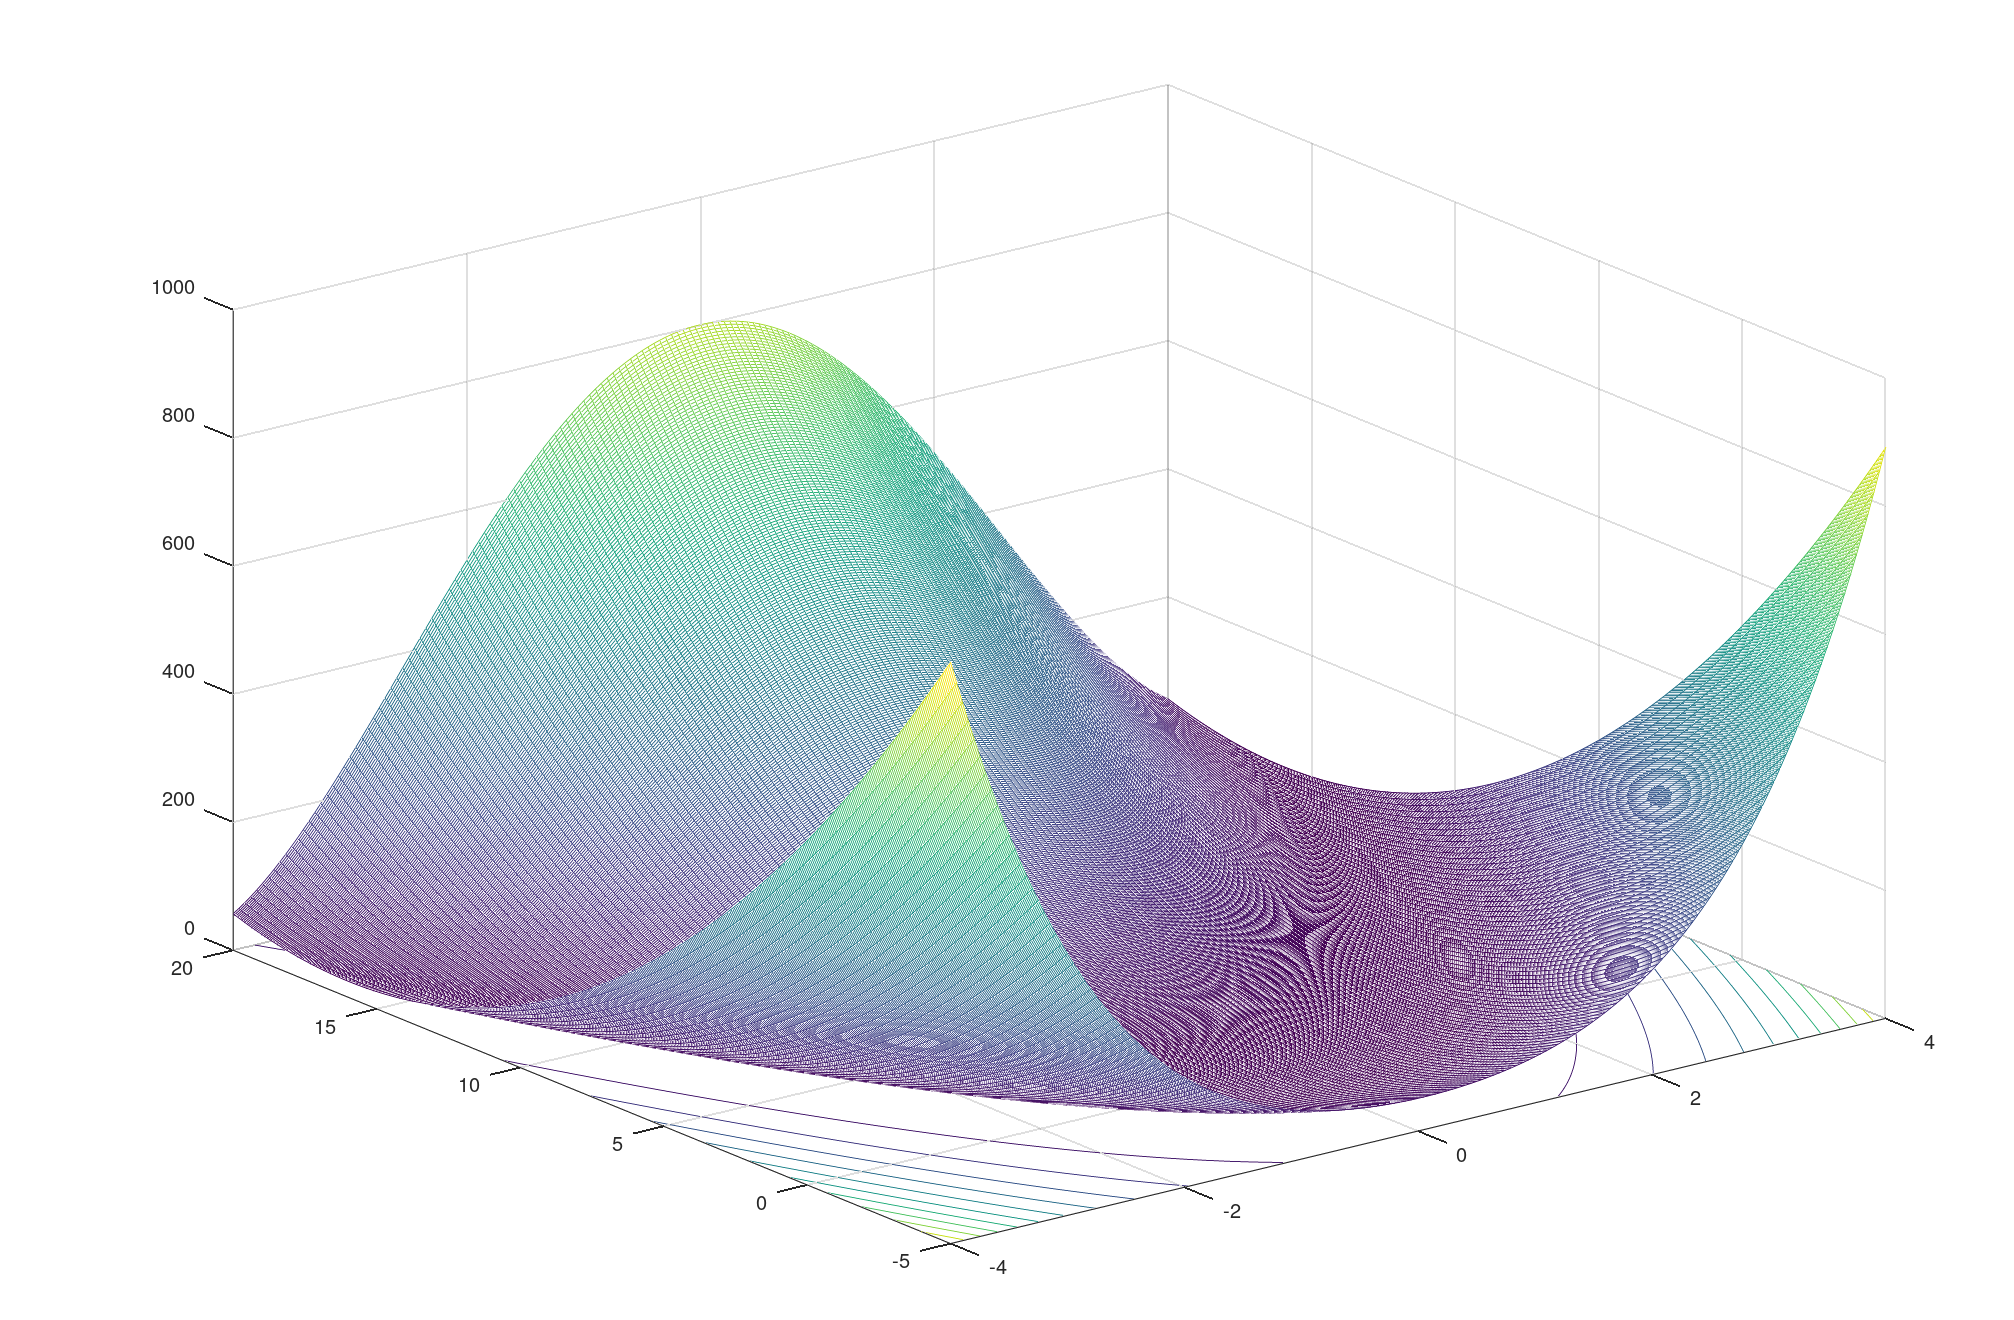
\includegraphics[width=\textwidth]{rosenbrock3D}
        \caption{Visualisation de la fonction de Rosenbrock en 3D}
    \end{subfigure}
    \begin{subfigure}[h]{0.49\textwidth}
        \centering
        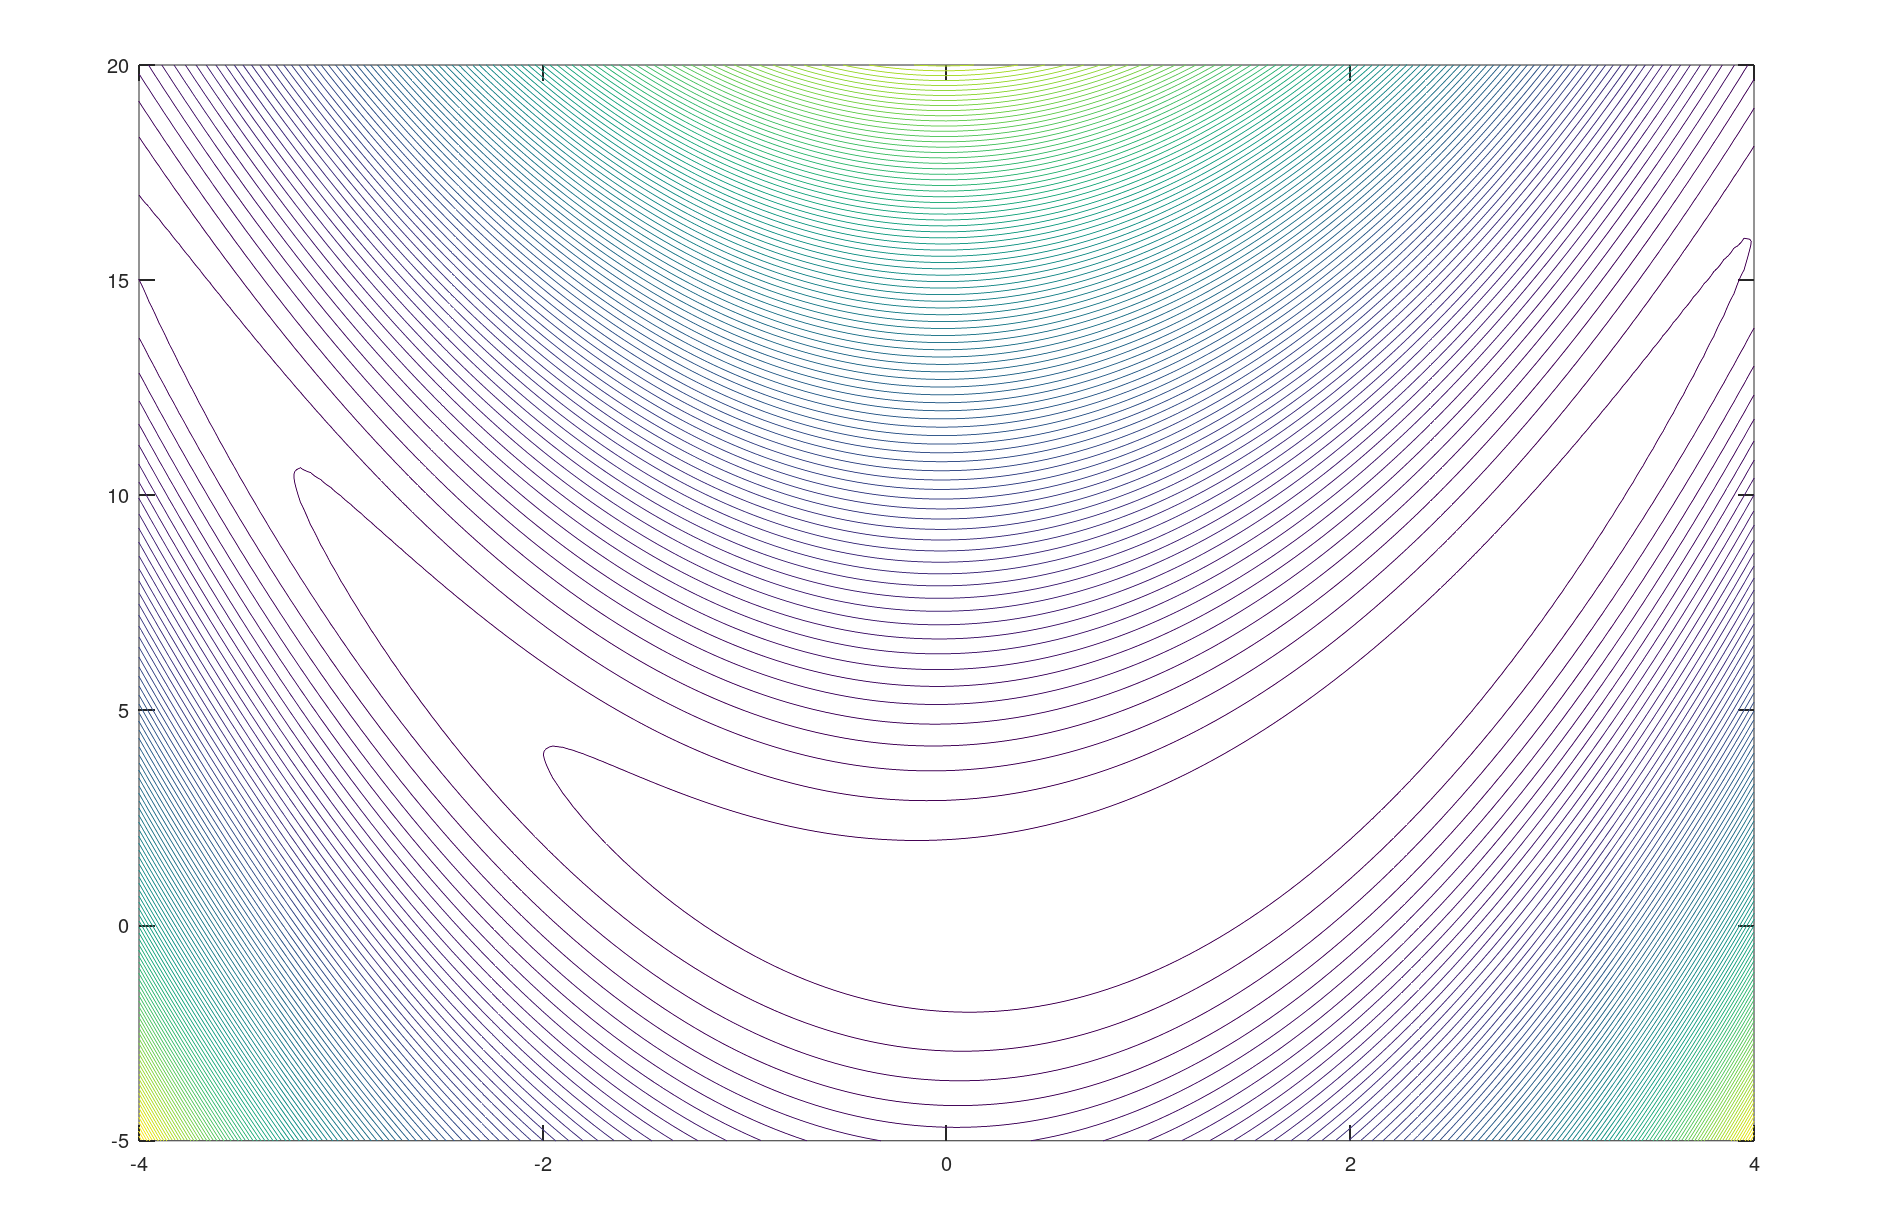
\includegraphics[width=\textwidth]{contourRosenbrock}
        \caption{Visualisation des lignes de niveaux de la fonction}
    \end{subfigure}
\end{figure}

\subsection{Minimisation par descente itérative}

\begin{enumerate}
    \item{
            Pour commencer, on utilise la méthode de descente de plus forte pente avec un pas fixe.
            On obtient alors en 1000 itérations les différents figures : 
            \begin{figure}[H]
                \centering
                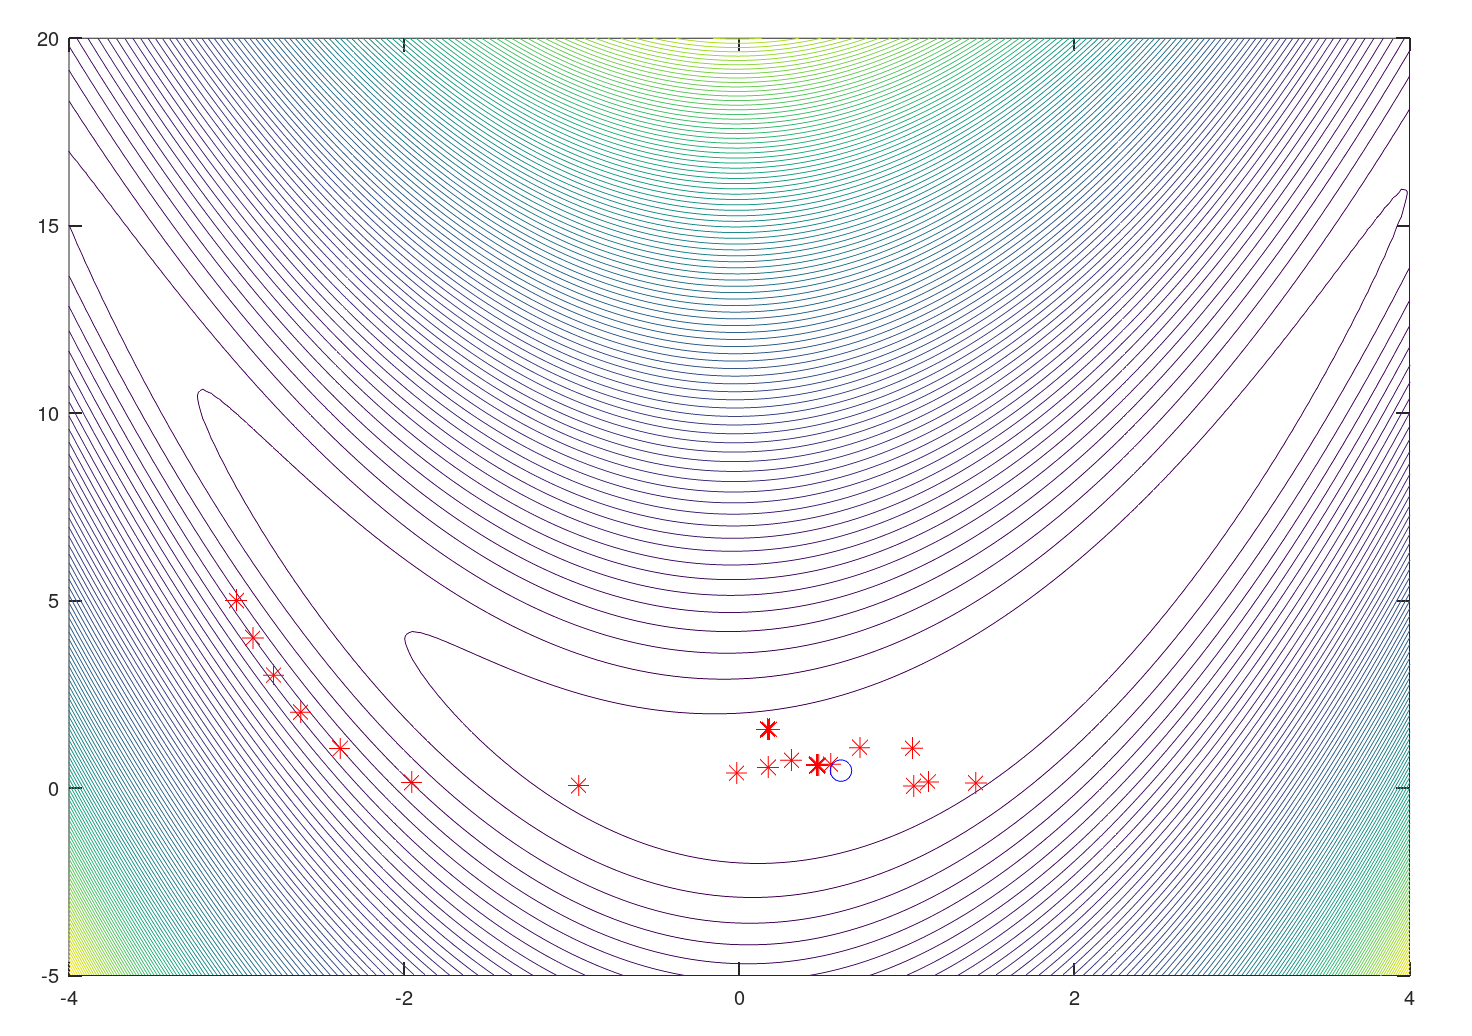
\includegraphics[width=7cm, height=4cm]{pasFixe1}
                \caption{Descente de pas 1}
            \end{figure}

            \begin{figure}[H]
                \centering
                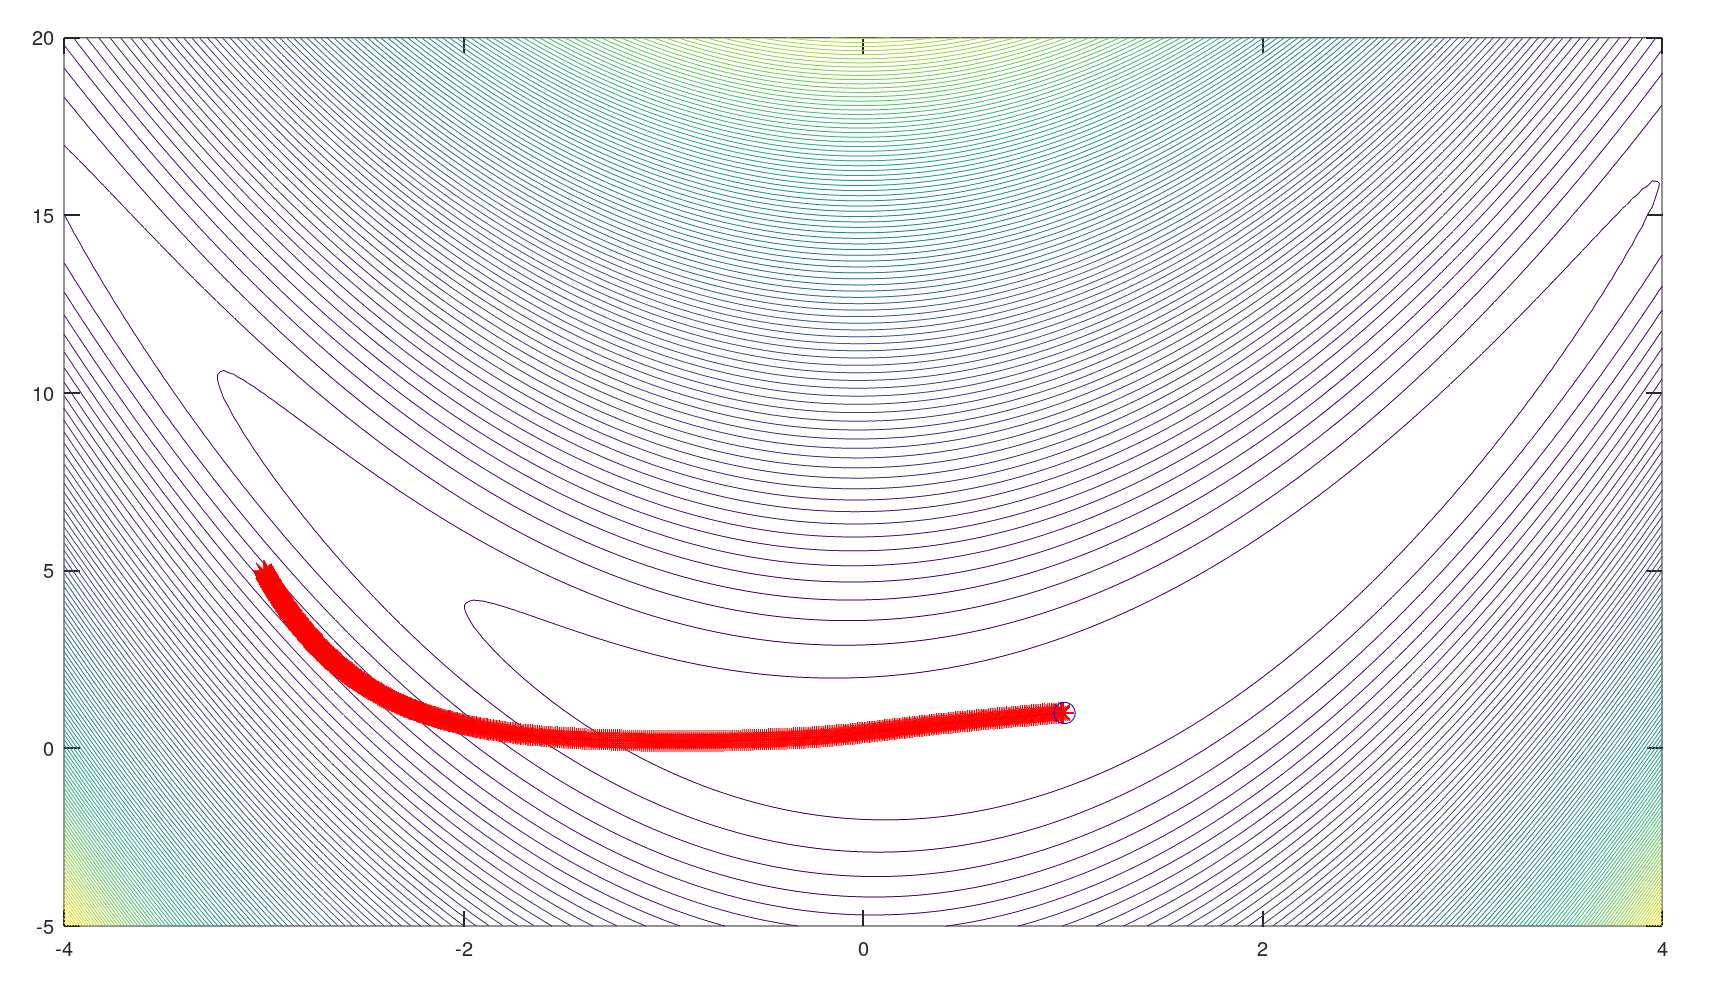
\includegraphics[width=7cm, height=4cm]{pasFixe10moins2}
                \caption{Descente de pas $10^{-2}$}
            \end{figure}

            \begin{figure}[H]
                \centering
                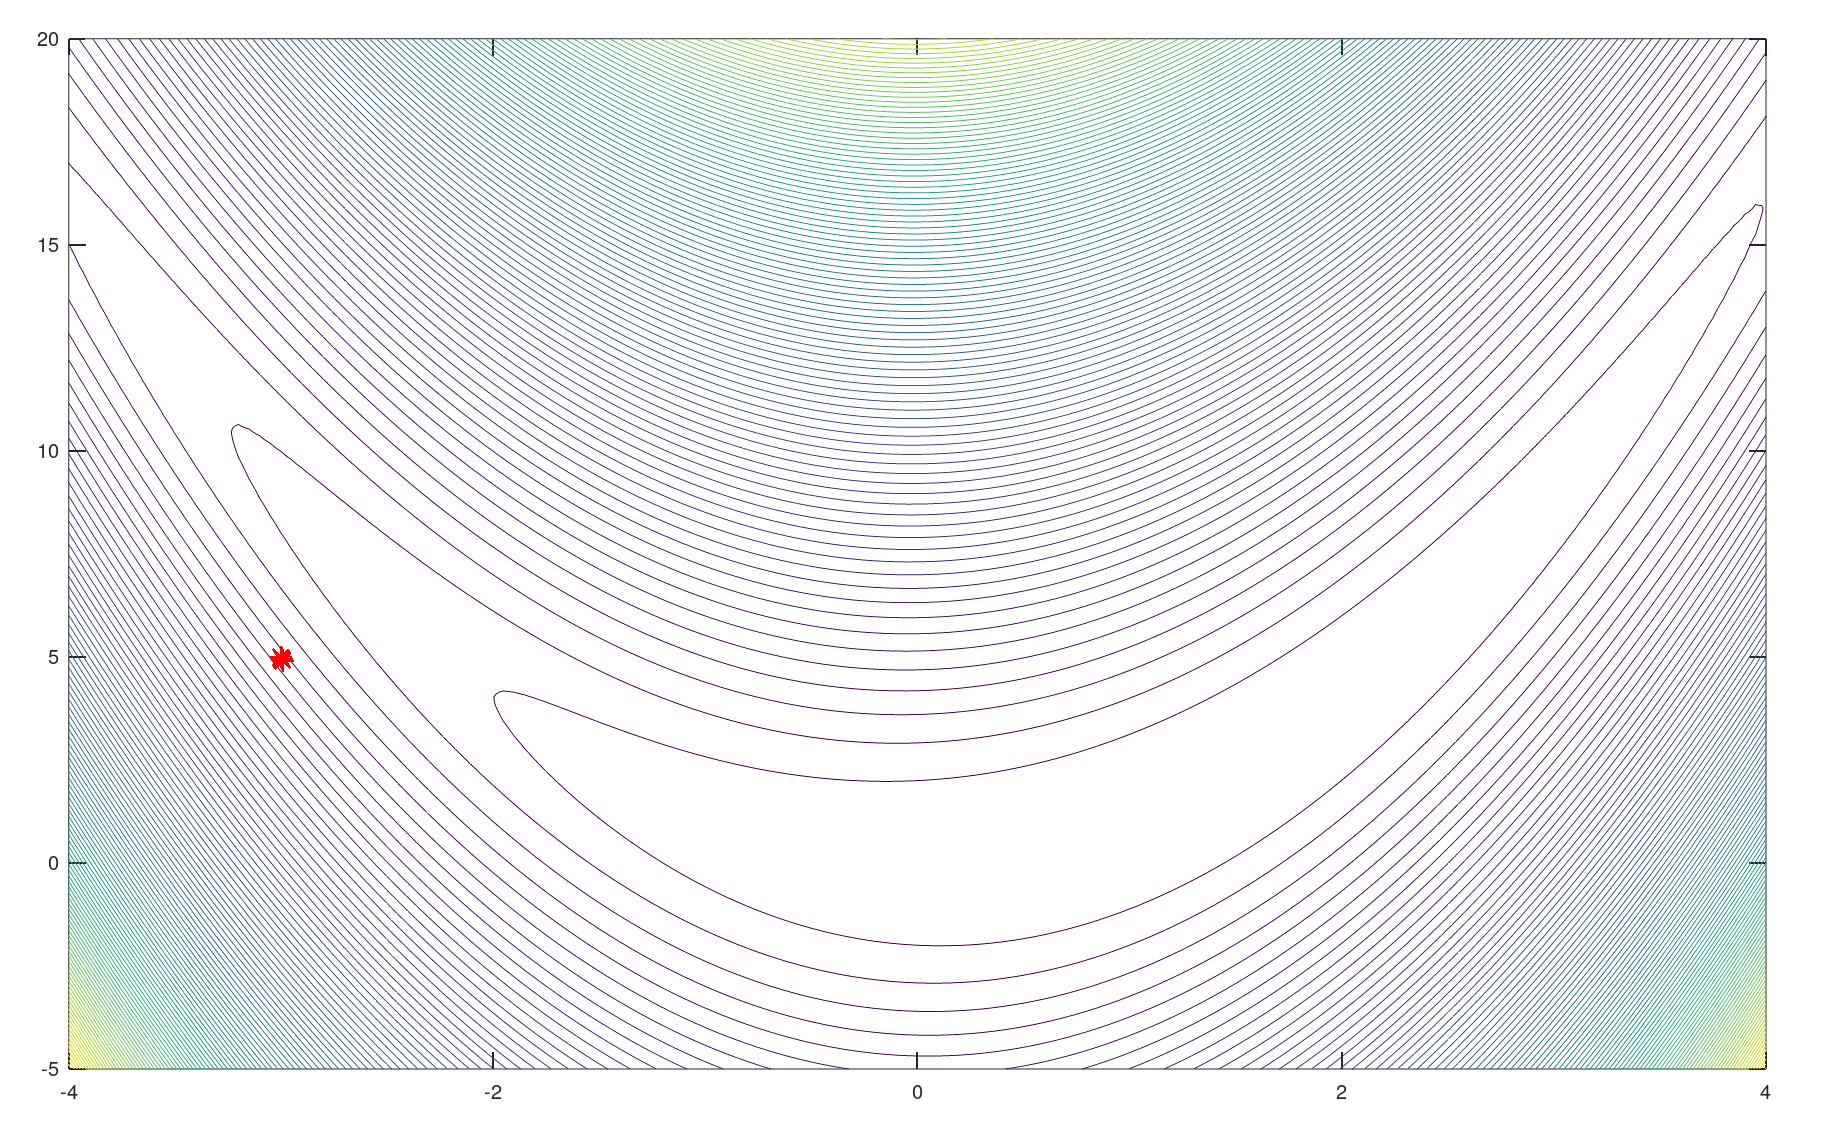
\includegraphics[width=7cm, height=4cm]{pasFixe10moins4}
                \caption{Descente de pas $10^{-4}$}
            \end{figure}

            On remarque que :
            \begin{itemize}
                \item{Avec le pas de $10^{-4}$, les 1000 itérations ne sont pas suffisante pour tendre vers $ x_h$}
                \item{Pour les deux autres valeurs du pas, la méthode converge vers $x_h$ mais avec le pas de 1, la méthode converge bien plus rapidement qu'avec le pas de $10^{-2}$.}
            \end{itemize}
        }

    \item{On ajoute alors une recherche de pas par une technique de rebroussement avec un taux $\beta = 0.75$ pour assurer la condition d'Armijo avec $c=10^{-4}$.

            \begin{figure}[H]
                \centering
                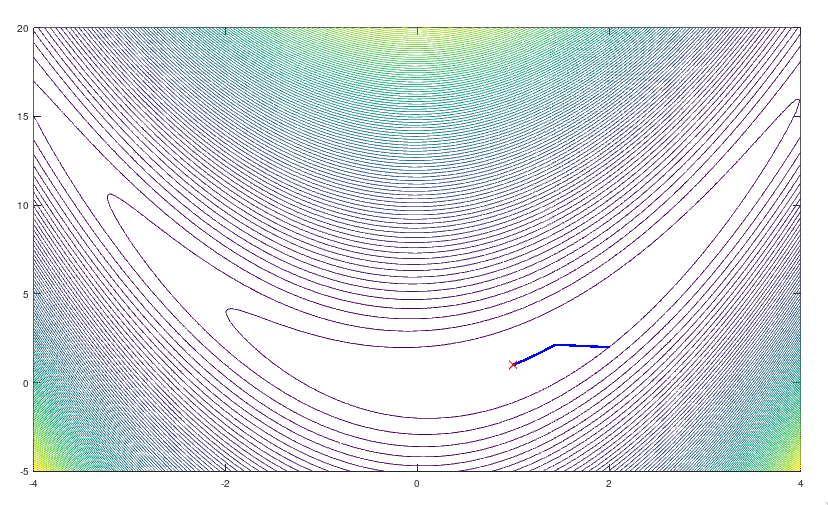
\includegraphics[width=7cm, height=4cm]{pasVar}
                \caption{technique de rebroussement}
            \end{figure}

            On observe alors que le pas varie effectivement au cours des itérations, de sorte à assurer la
            condition d'Armijo, ce qui garantit une décroissance suffisante et permet donc de ne pas avoir à se
            soucier des problèmes vus plus haut (pas trop faible ou trop élevé). Cependant, cette méthode est
            plus stable mais nécessite plus de calculs que pour la méthode du pas fixe, elle est par exemple 
            bien plus lente que la méthode de pas fixe avec un pas de 1 pour cet exemple précis.
        }

        \setcounter{enumi}{3}
    \item{
            Pour la valeur : $x_0 = (4, 4)$, on obtient les tracés suivants :

            \begin{figure}[H]
                \centering
                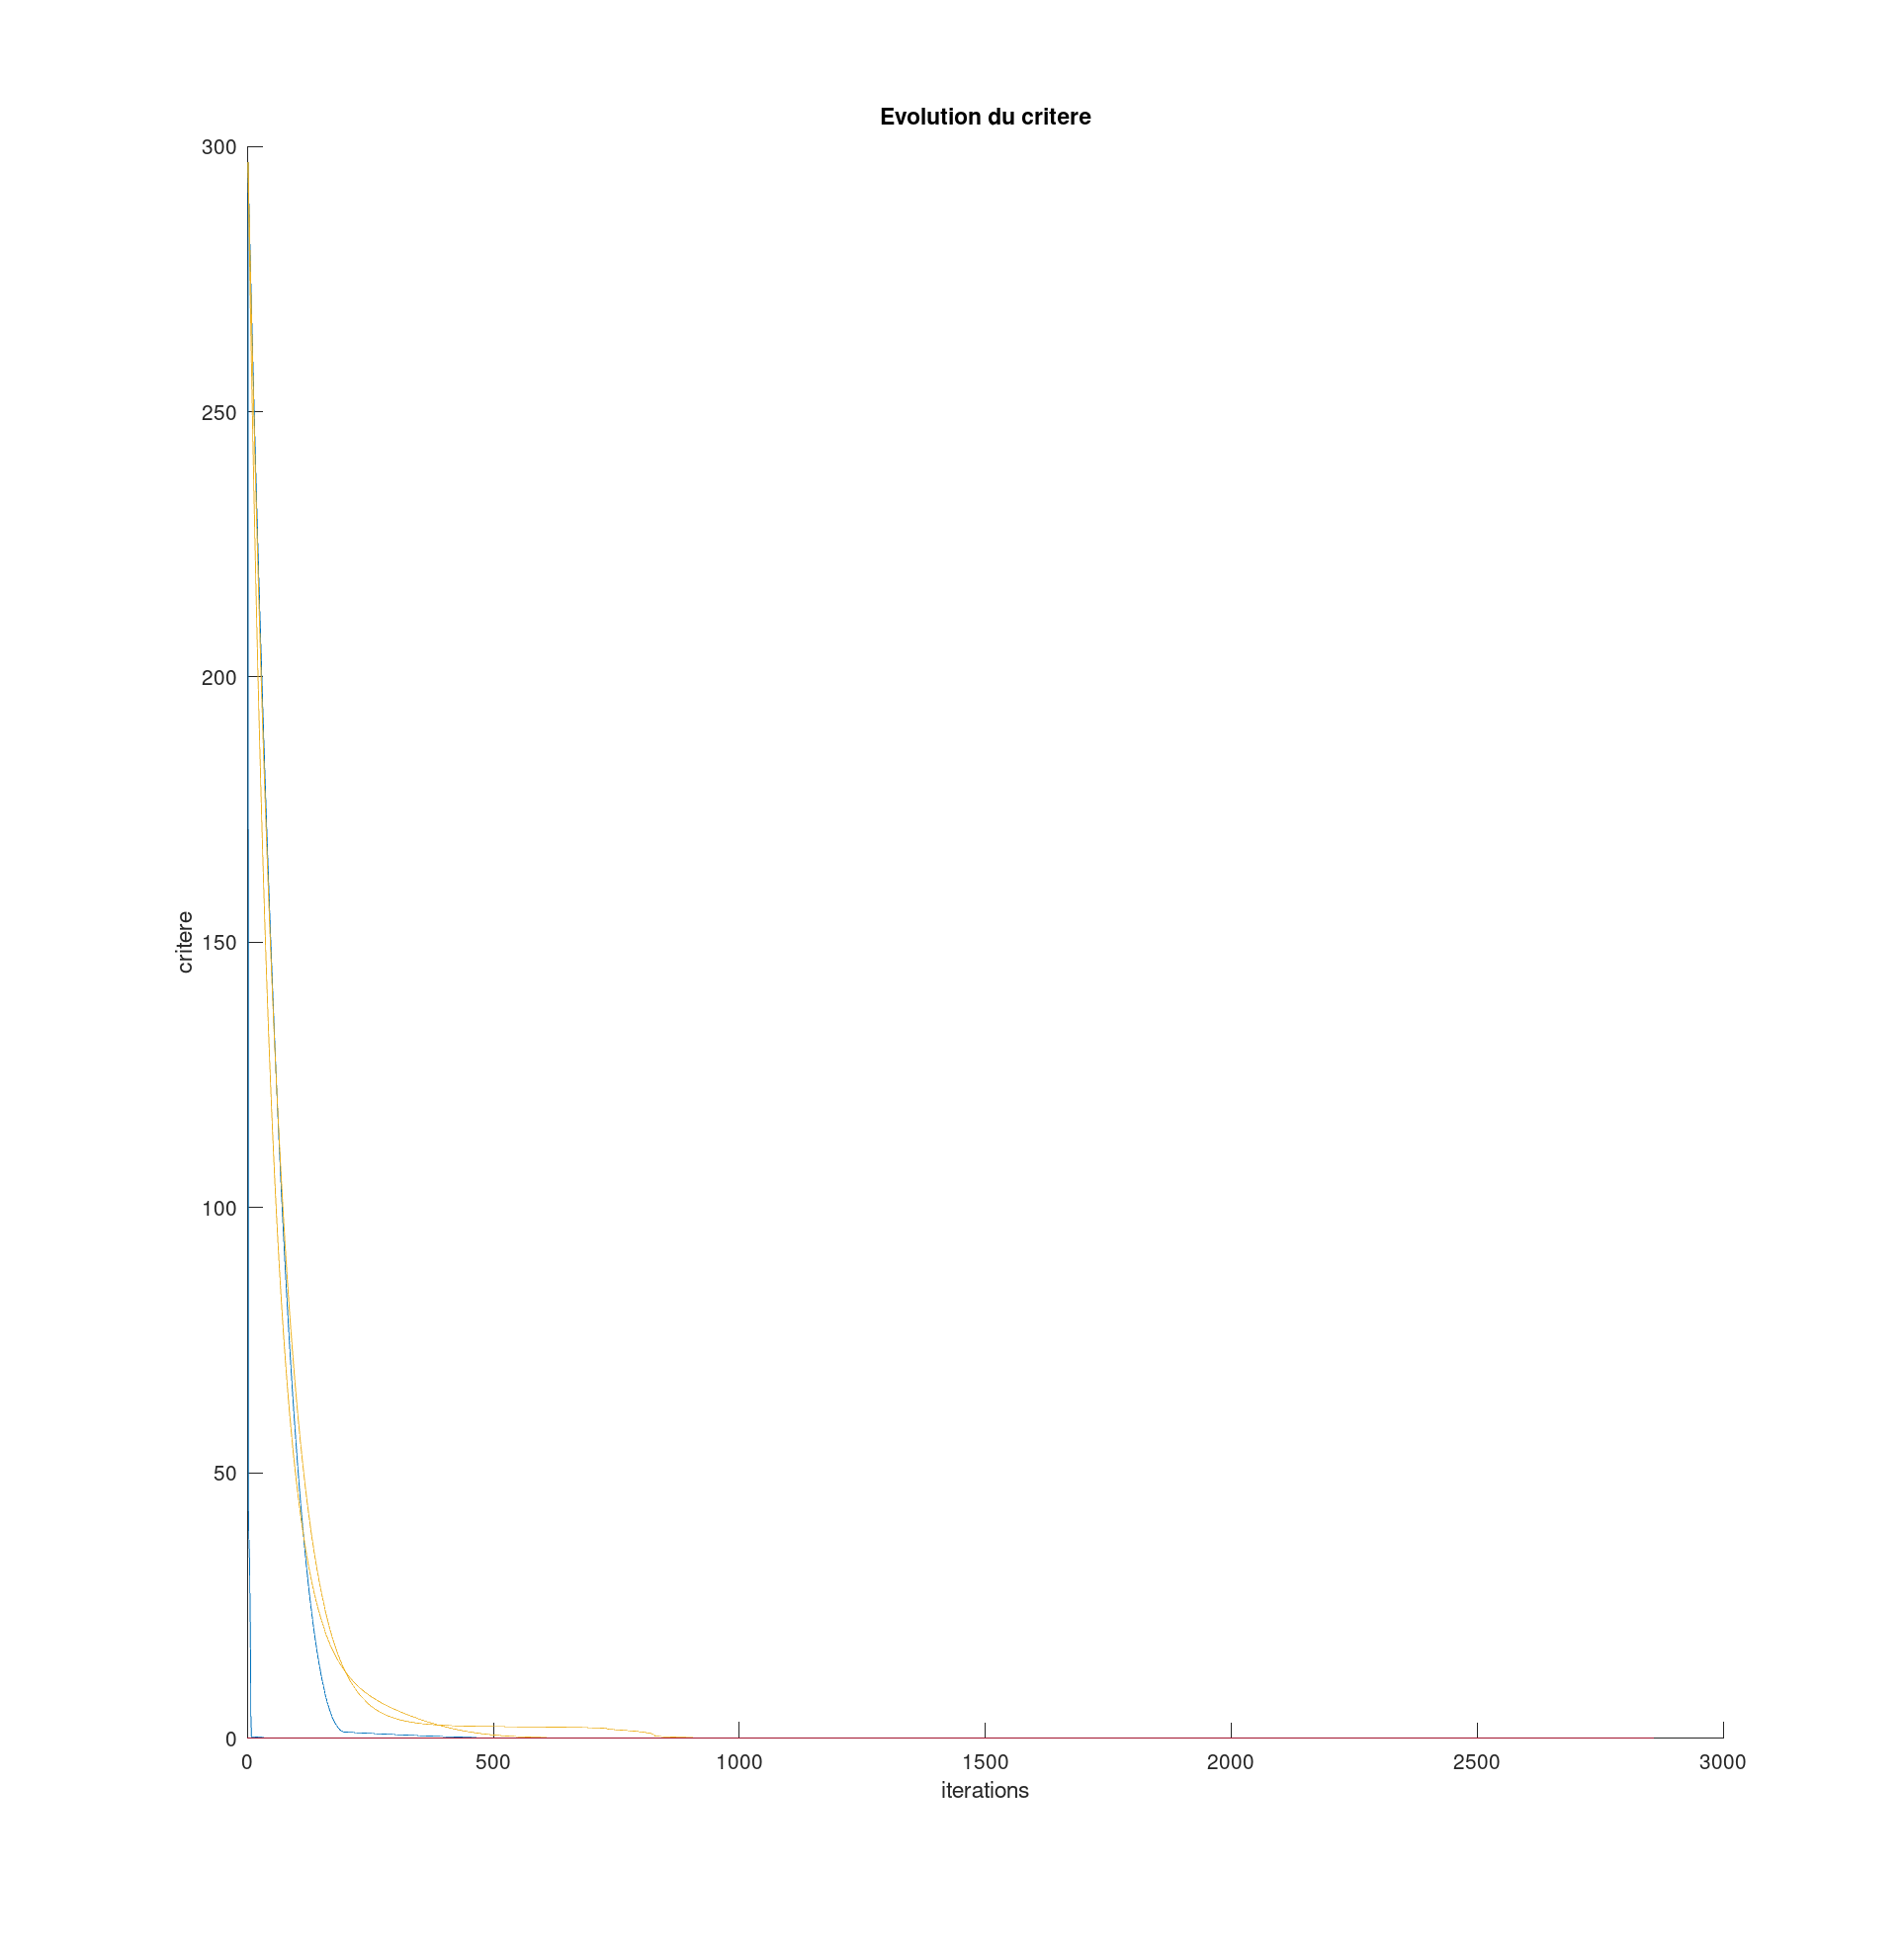
\includegraphics[width=0.5\textwidth]{critere}
                \caption{Évolution du critère}
            \end{figure}

            \begin{figure}[H]
                \centering
                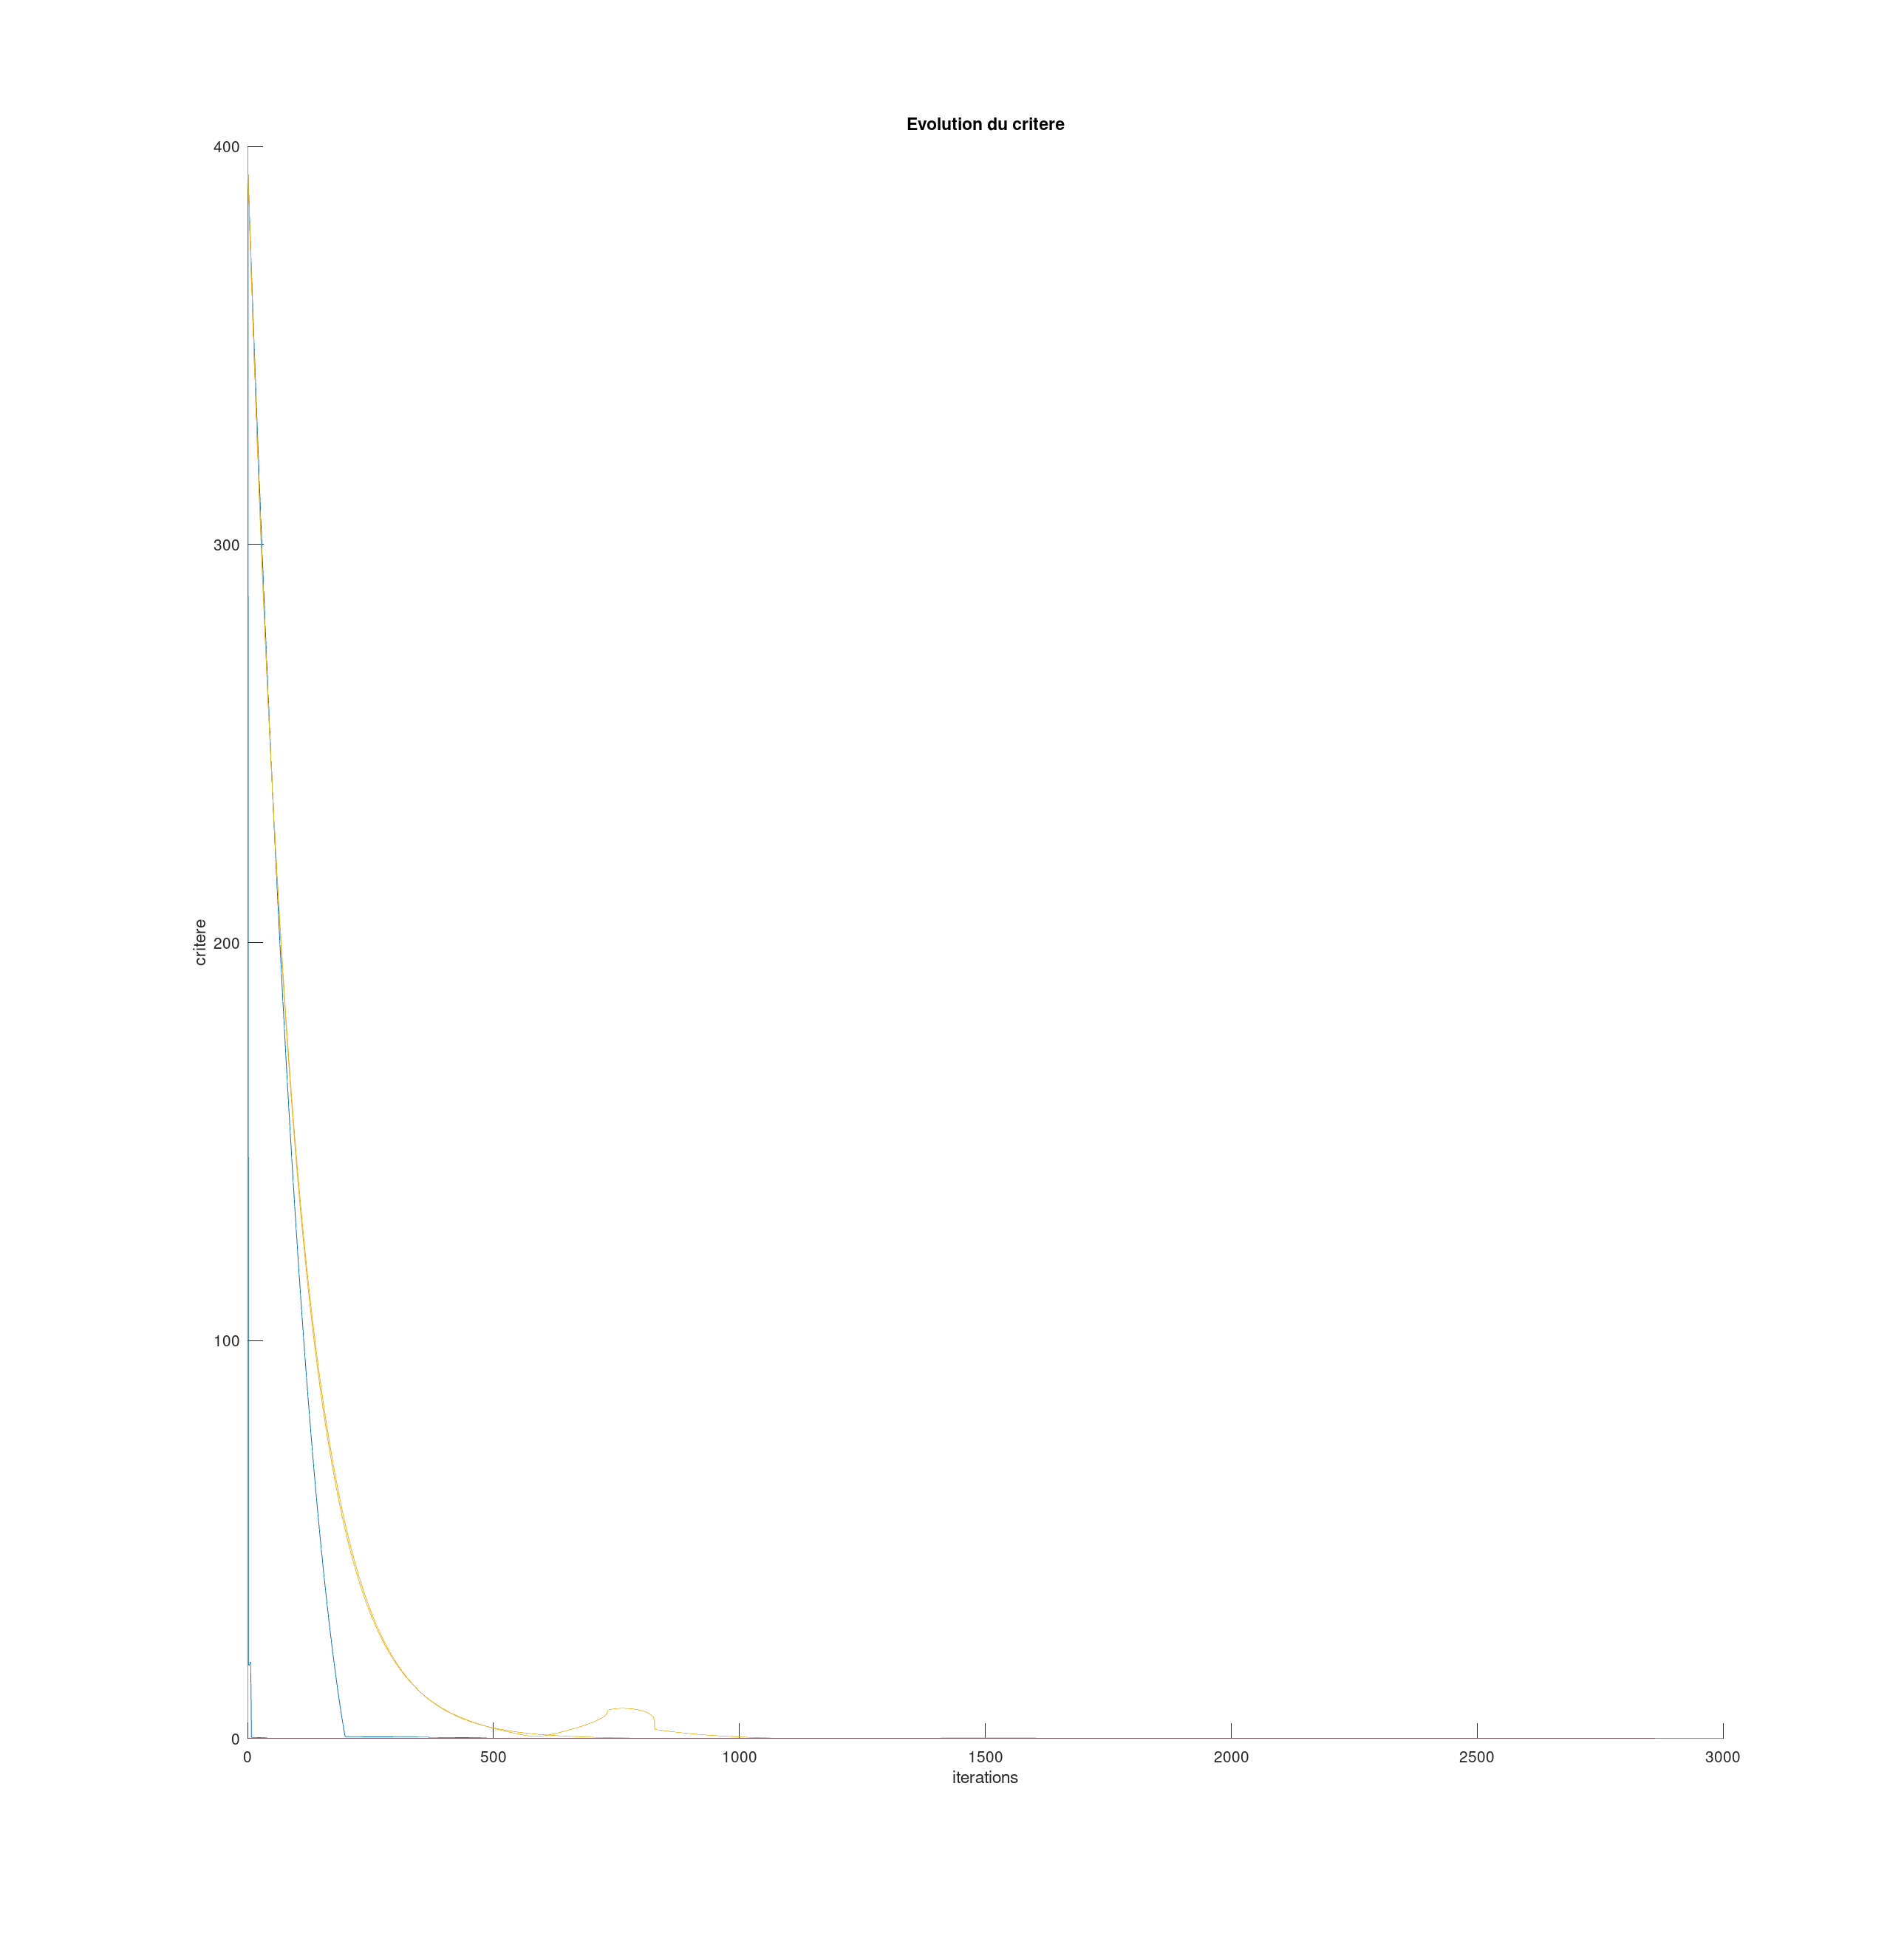
\includegraphics[width=0.5\textwidth]{gradient}
                \caption{Évolution de la norme du gradient}
            \end{figure}

            Pour la valeur : $x_0 = (5, 10)$ et avec un pas variable, on obtient les tracés suivants :

            \begin{figure}[H]
                \centering
                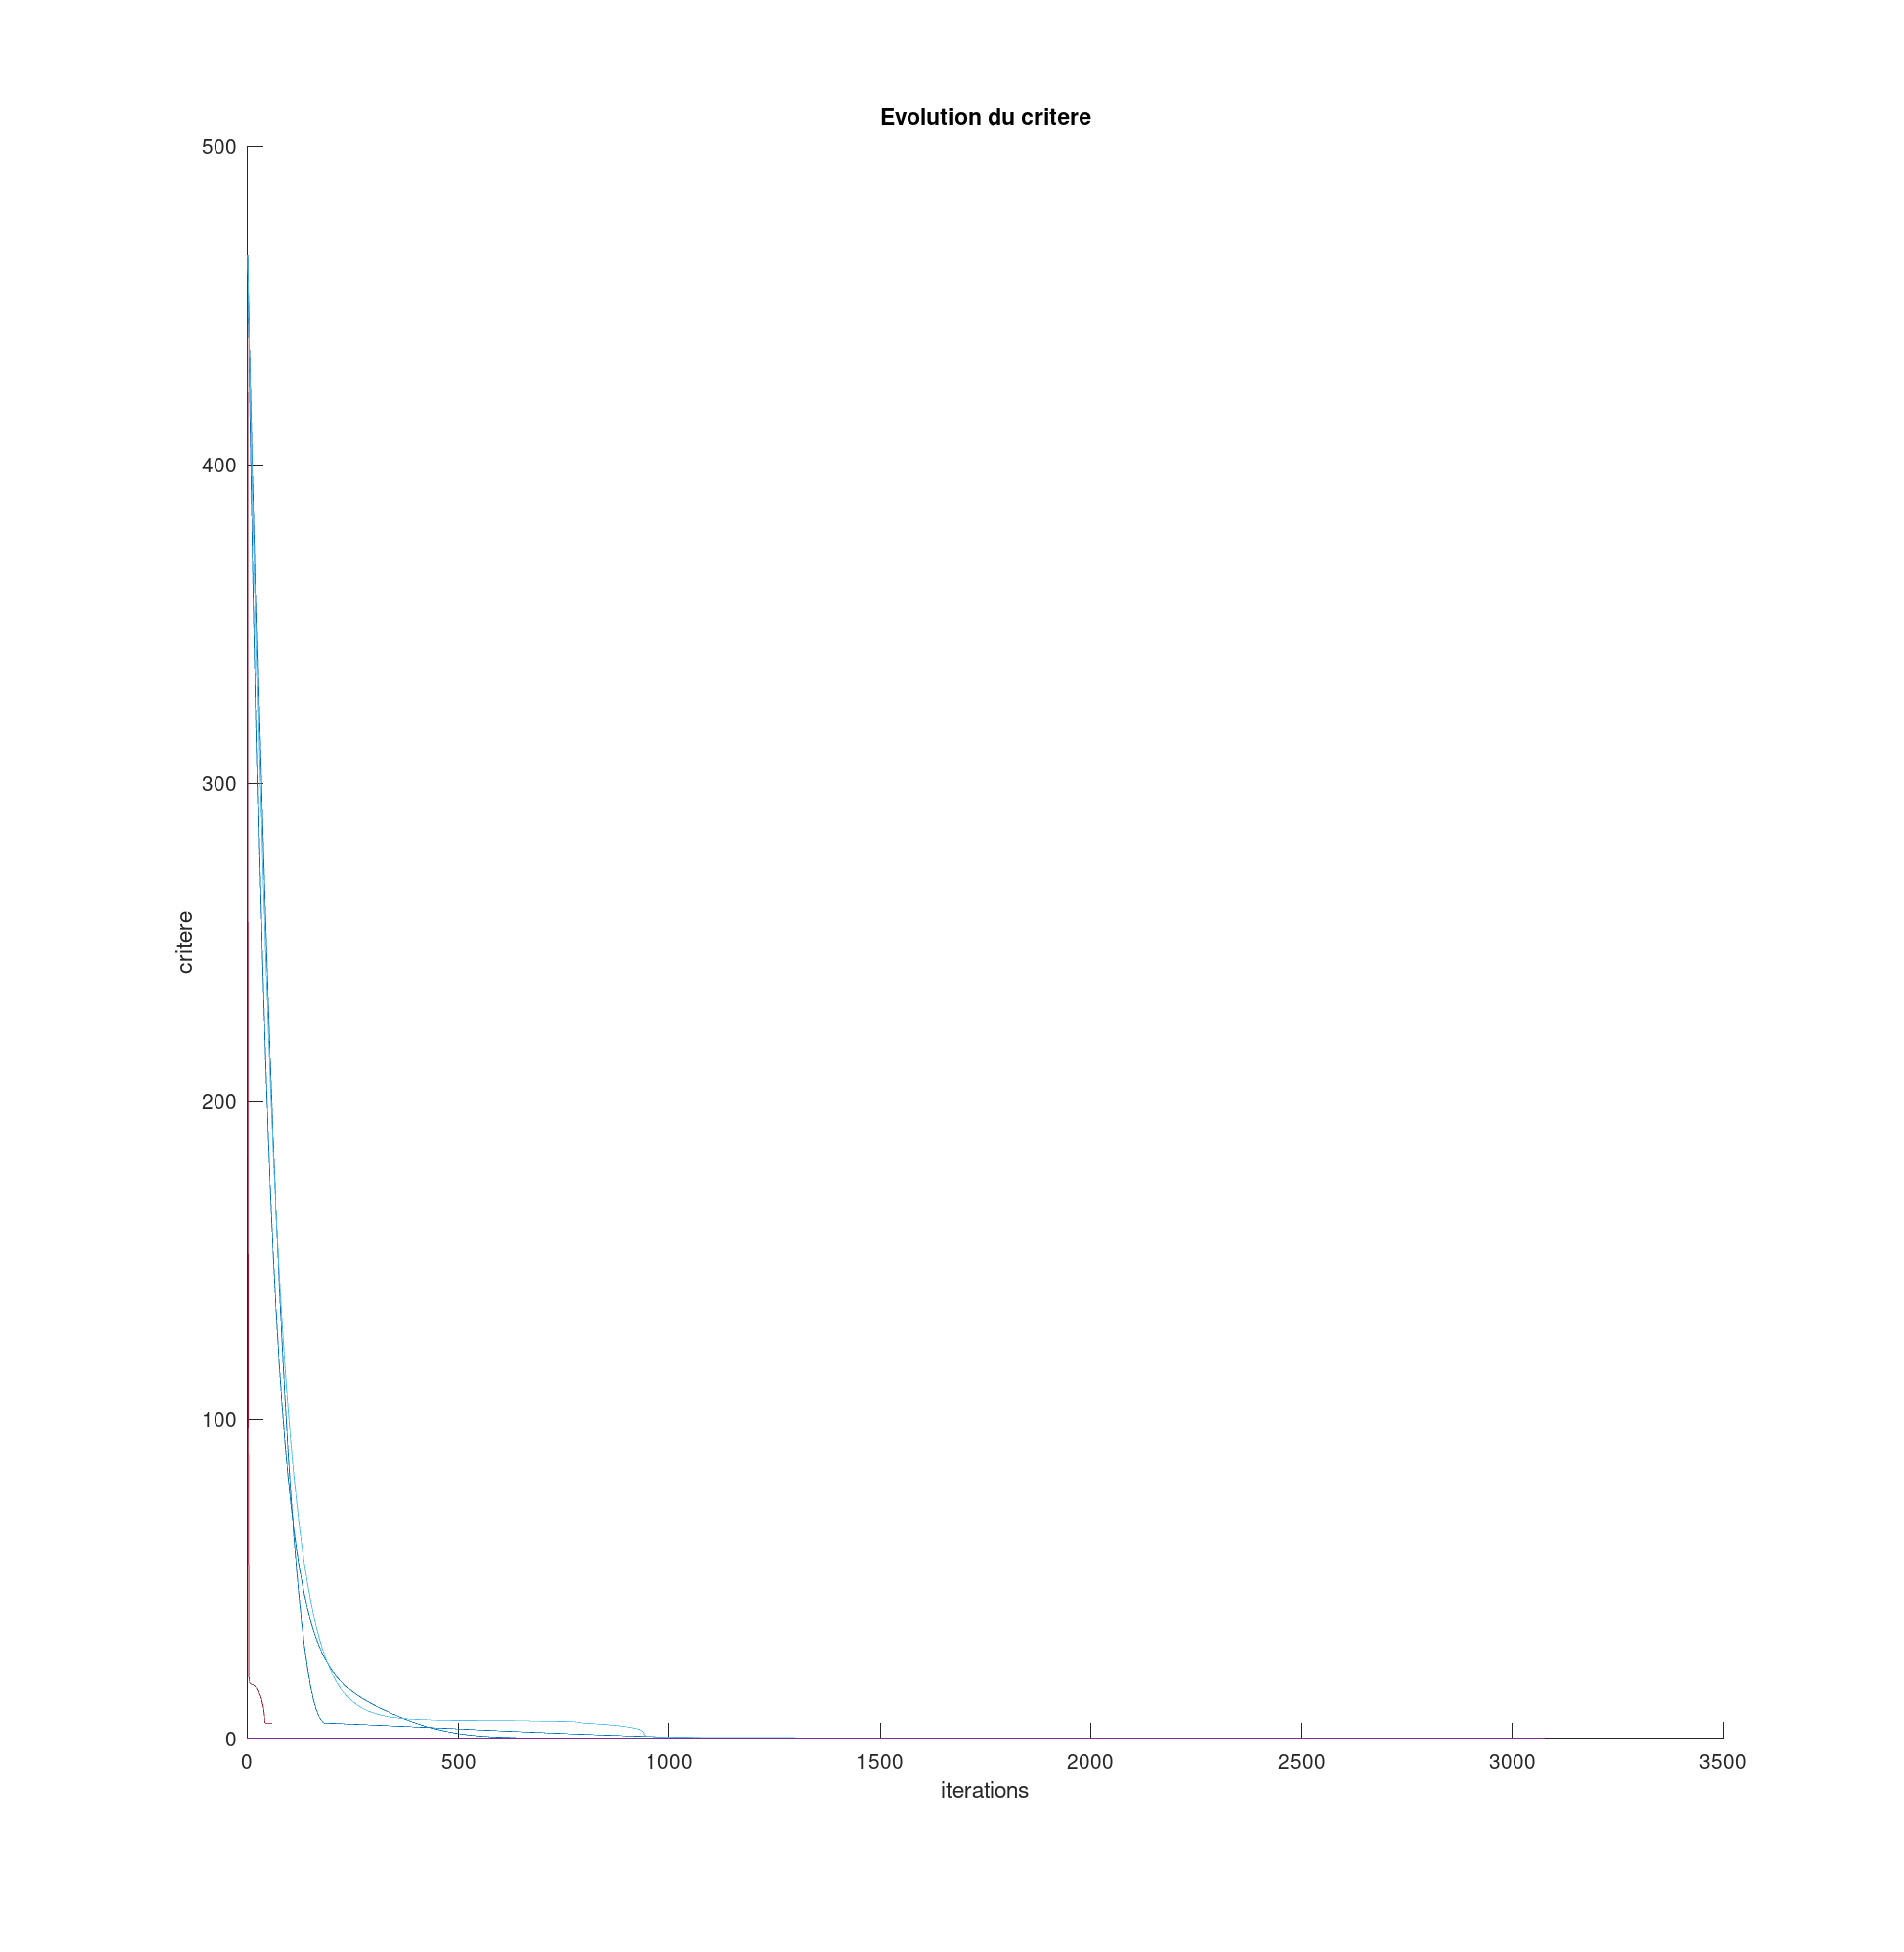
\includegraphics[width=0.5\textwidth]{critere2}
                \caption{Évolution du critère}
            \end{figure}

            \begin{figure}[H]
                \centering
                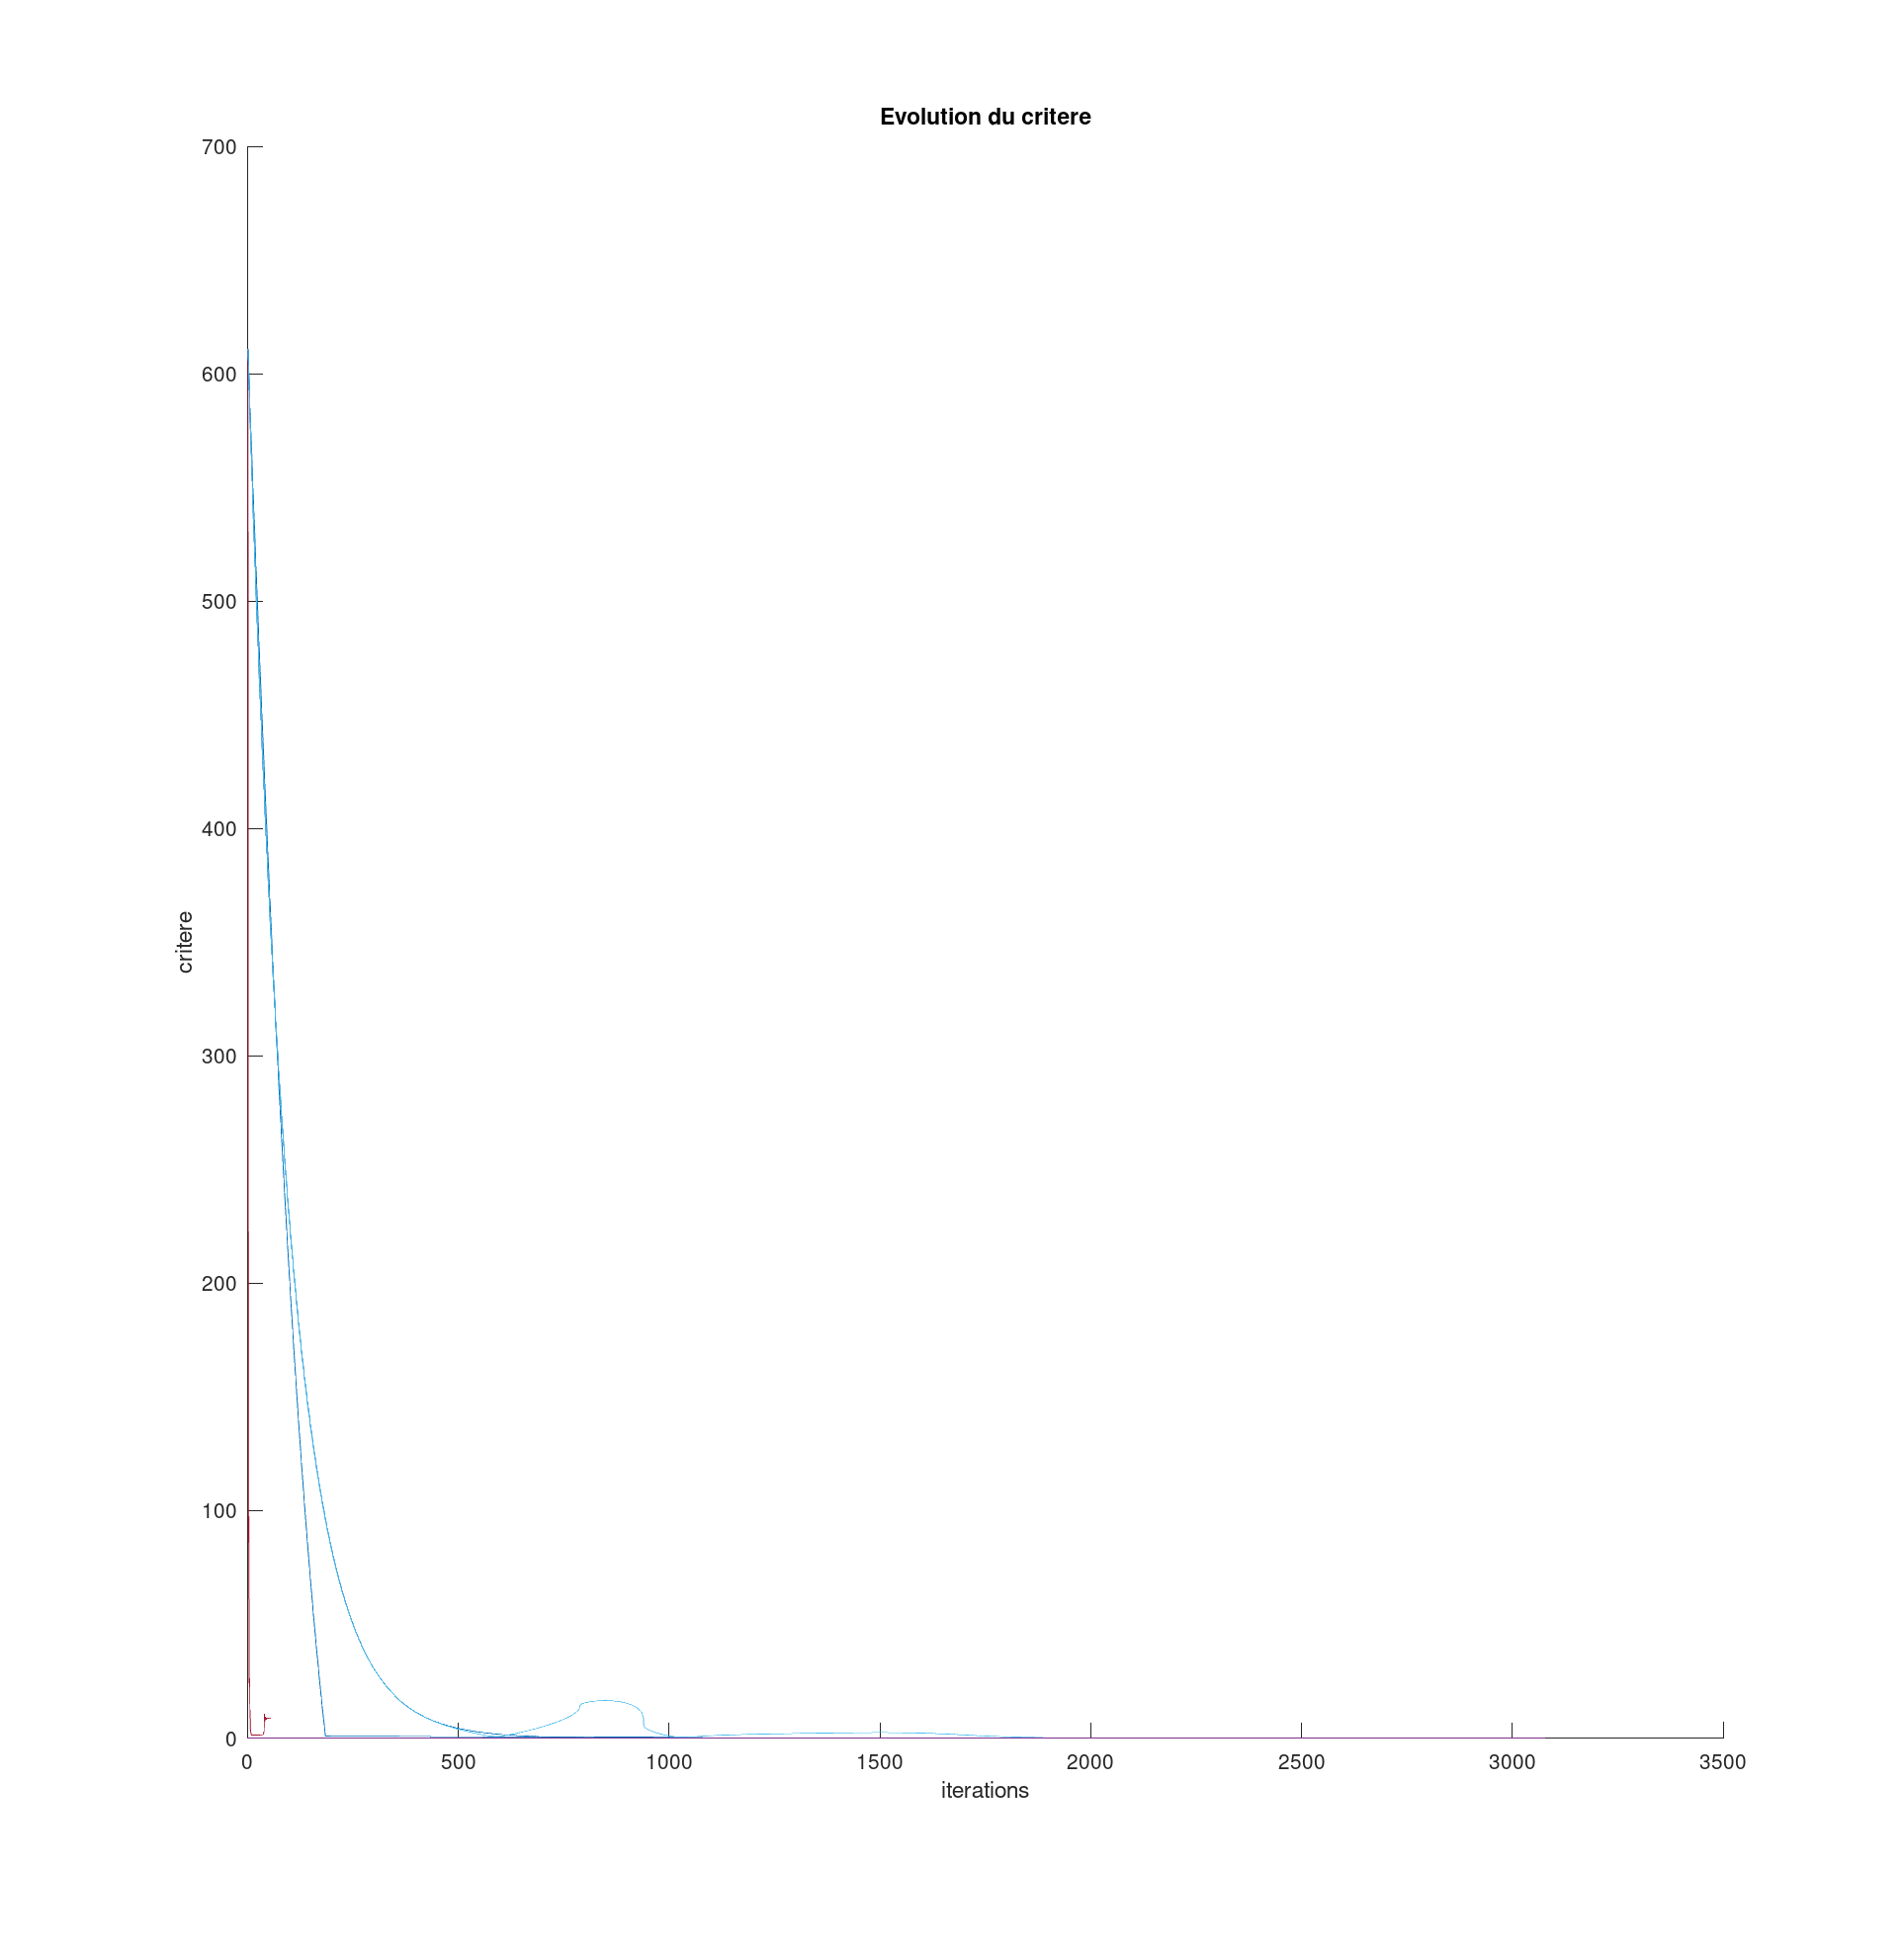
\includegraphics[width=0.5\textwidth]{gradient2}
                \caption{Évolution de la norme du gradient}
            \end{figure}

            On observe que pour ces 4 tracés le critère et le gradient s'annulent
            rapidement pour chaque méthode, il faudrait choisir des valeurs de tolérance plus
            adaptées pour gagner en temps d'exécution, quitte à être légèrement moins précis.
            Pour comparer les performances de chaque méthode représentons le nombre d'itérations
            et le temps d'exécution dans un tableau :

            Pour $x_0 = (4,4)$ :

            \begin{table}[H]
                \begin{tabularx}{\textwidth}{ |l|X|X| }
                    \hline
                    Méthode & Nombre d'itérations & Temps (s) \\
                    \hline
                    Descente de plus forte pente & 911 & 0.51 \\
                    \hline
                    Gradient conjugué & 451  & 0.18 \\
                    \hline
                    Newton & 1989 & 0.37 \\
                    \hline
                    BFGS & 2862 & 0.75 \\
                    \hline
                \end{tabularx}
            \end{table}

            Pour $x_0 = (5,10)$ :

            \begin{table}[H]
                \begin{tabularx}{\textwidth}{ |l|X|X| }
                    \hline
                    Méthode & Nombre d'itérations & Temps (s) \\
                    \hline
                    Descente de plus forte pente & 1526 & 0.70 \\
                    \hline
                    Gradient conjugué & x & x \\
                    \hline
                    Newton & 2043 & 0.64 \\
                    \hline
                    BFGS & 3000 & 1.30 \\
                    \hline
                \end{tabularx}
            \end{table}

            On remarque alors que :

            \begin{itemize}
                \item{Pour la première valeur de $x_0$, la méthode du gradient conjuguée est la
                    plus performante que ce ce soit en temps de calcul ou en nombre d'itérations}
                \item{Mais la méthode du gradient conjuguée ne converge pas vers $x_h$ pour une
                    position initiale plus éloignée.}
                \item{Les méthodes de Newton et BFGS sont celles nécessitant le plus d'itérations}
                \item{La méthode de Newton est cependant plus rapide que celle du gradient de plus
                    forte pente}
            \end{itemize}

        }

        \setcounter{enumi}{5}
    \item{
            Pour $x_0 = (4,4)$ :

            \begin{table}[H]
                \begin{tabularx}{\textwidth}{ |l|X|X| }
                    \hline
                    Méthode & Nombre d'itérations & Temps (s) \\
                    \hline
                    Gauss-Newton & 1603 & 0.31 \\
                    \hline
                    levenberg-marquardt & 1594 & 0.33 \\
                    \hline
                \end{tabularx}
            \end{table}

            Pour $x_0 = (5,10)$ :

            \begin{table}[H]
                \begin{tabularx}{\textwidth}{ |l|X|X| }
                    \hline
                    Méthode & Nombre d'itérations & Temps (s) \\
                    \hline
                    Gauss-Newton & 1622 & 0.32 \\
                    \hline
                    levenberg-marquardt & 1607 & 0.35 \\
                    \hline
                \end{tabularx}
            \end{table}

            On remarque alors que :

            \begin{itemize}
                \item{Les deux méthodes convergent bien vers $x_h$ pour les deux valeurs de $x_0$.}
                \item{Les performances de ces deux méthodes sont très similaires pour les
                        deux valeurs de $x_0$, ce qui n'est pas le cas des autres méthodes et
                    qui représente un avantage important.}
                \item{Ce sont les méthodes les plus rapides pour la deuxième valeur de $x_0$ et
                    la deuxième plus rapide pour la première valeur de $x_0$.}
                \item{La méthode de levenberg-marquardt nécessite le choix d'une valeur pour
                        un paramètre. Dans ce cas ci, nous obtenons des résultats satisfaisant
                        uniquement pour des valeurs très faibles de $\lambda$, la méthode est 
                    alors quasiment équivalente à celle de Gauss-Newton.}
            \end{itemize}
        }

\end{enumerate}

\newpage
\section{Ajustement d'une courbe non-linéaire}
	On cherche à minimiser la fonction objectif :	
	$$
		f_0( \alpha,\beta ) =  \frac{ 1}{2}  \sum_{i=1}^{N} ( R_i - \beta E_i^{-\alpha} )^2
	$$
\begin{enumerate}
    \item{
    	Après calcul, on trouve :
	$$
	\nabla f(x) = \left[
                \begin{array}{c}
                    \sum_{i=1}^{N} \beta ln(E_i)E_i^{-\alpha} (R_i-\beta E_i^{-\alpha} )\\
                     - \sum_{i=1}^{N} E_i^{-\alpha} (R_i-\beta E_i^{-\alpha})
                \end{array}
            \right]
	$$
	
	$$
	  \nabla ^2f(x)=\left[
                \begin{array}{cc}
                    \sum_{i=1}^{N} \beta E^{-\alpha} ln(E_i)^2 (2\beta E_i^{-\alpha}-R_i) &  \sum_{i=1}^{N} E_i^{-\alpha}ln(E_i) (R_i -2\beta E_i^{-\alpha}) \\
                    \sum_{i=1}^{N} E_i^{-\alpha}ln(E_i) (R_i -2\beta E_i^{-\alpha}) &  \sum_{i=1}^{N} E_i^{-2\alpha}
                \end{array}
            \right]
	$$
    }
    
    \item{
    Pour les courbes de niveau, on la trace en echelle log pour $ 0< \alpha < 2$ et $ 0 < \beta <4$
    	\begin{figure}[H]
                \centering
                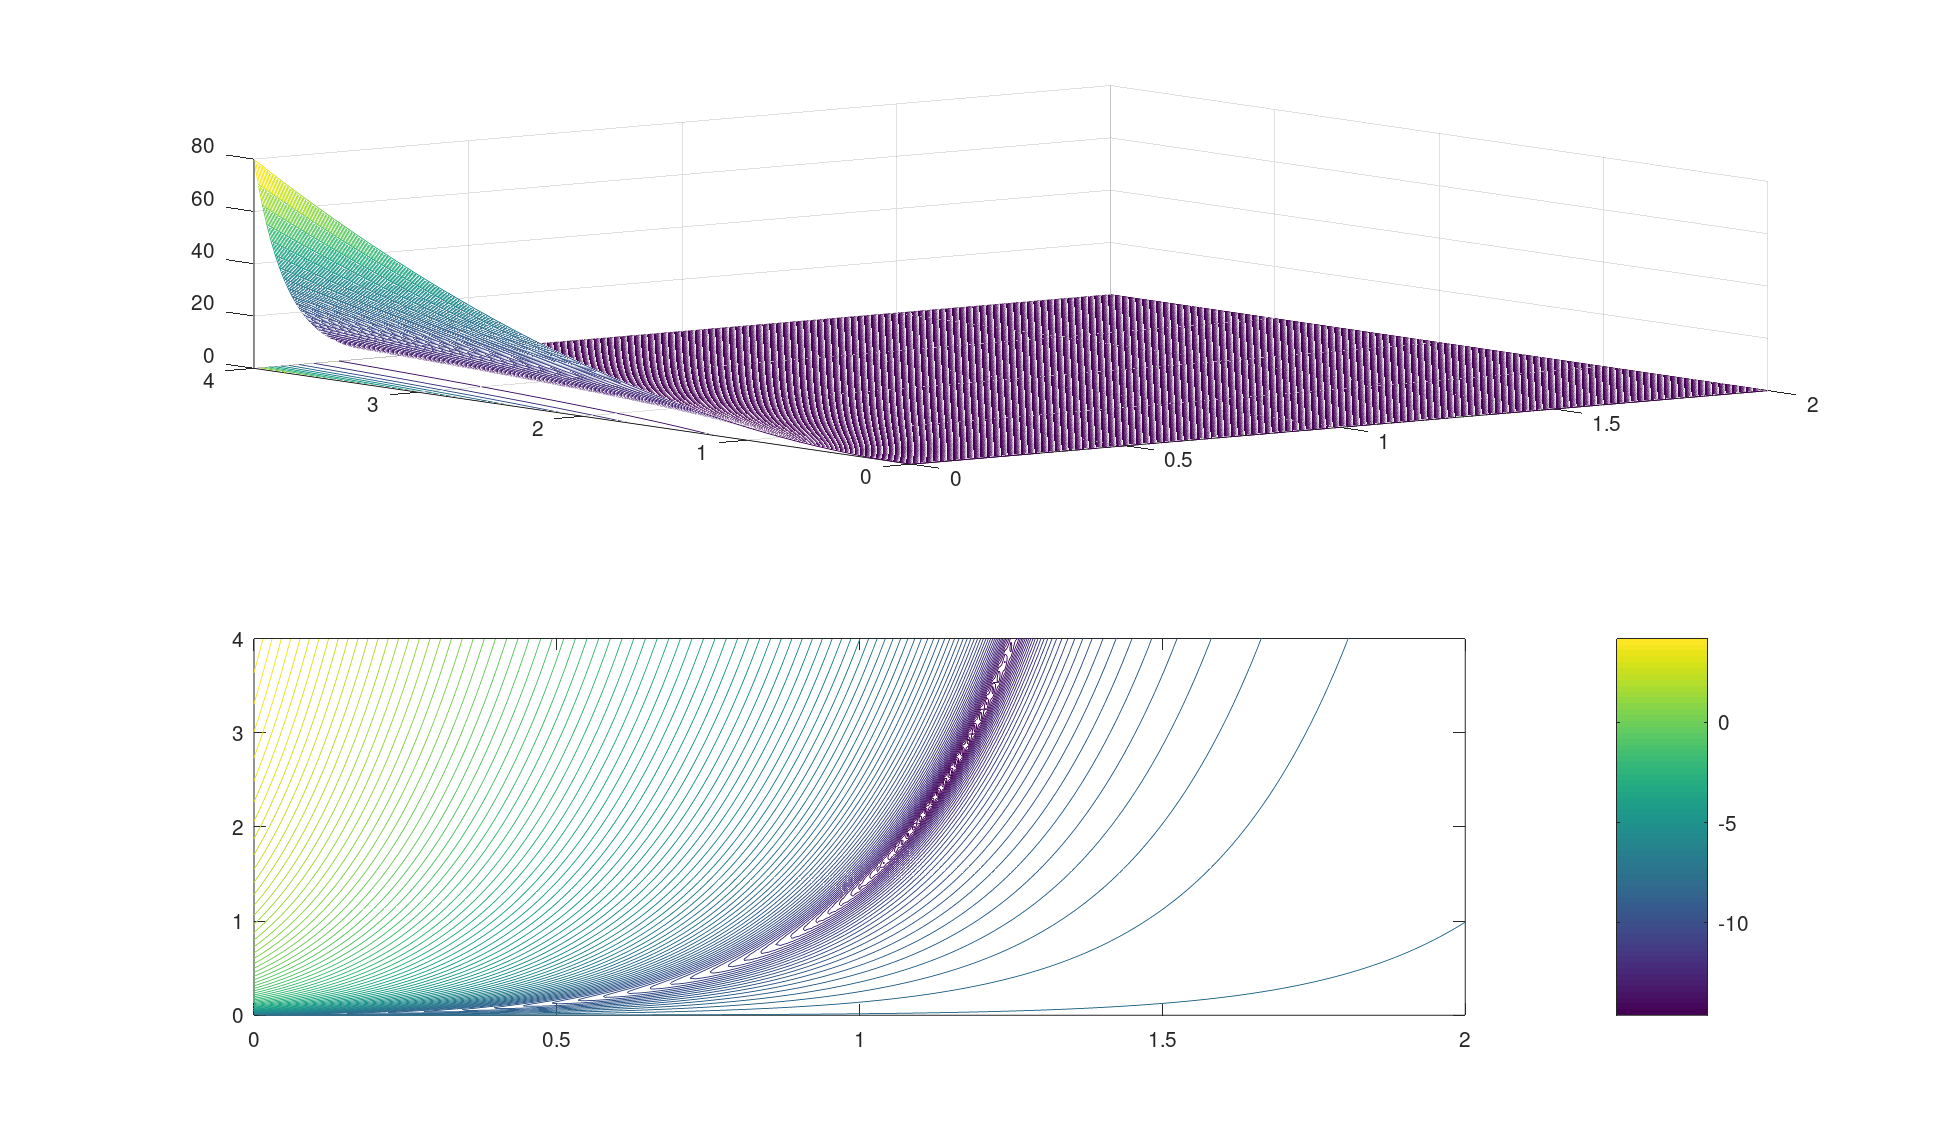
\includegraphics[width=0.7\textwidth]{contourExo2.png}
                \caption{Courbe de niveau du log-critère}
            \end{figure}
    }
    
    \item{Par la suite on applique les algorithmes vu à l'exercice 1 pour trouver les paramètres optimaux. On retrouve ainsi les résultats suivants :
    	\begin{figure}[H]
                \centering
                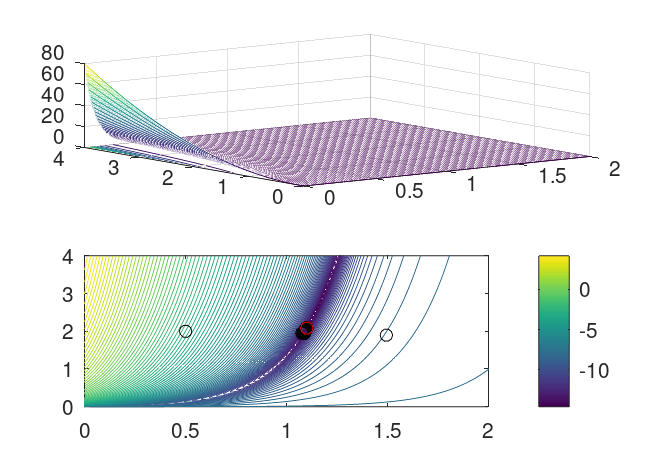
\includegraphics[width=0.7\textwidth]{contourExo2GradientVariable.png}
                \caption{Convergence pour une direction de plus forte pente avec pas variable}
            \end{figure}
            
            \begin{figure}[H]
                \centering
                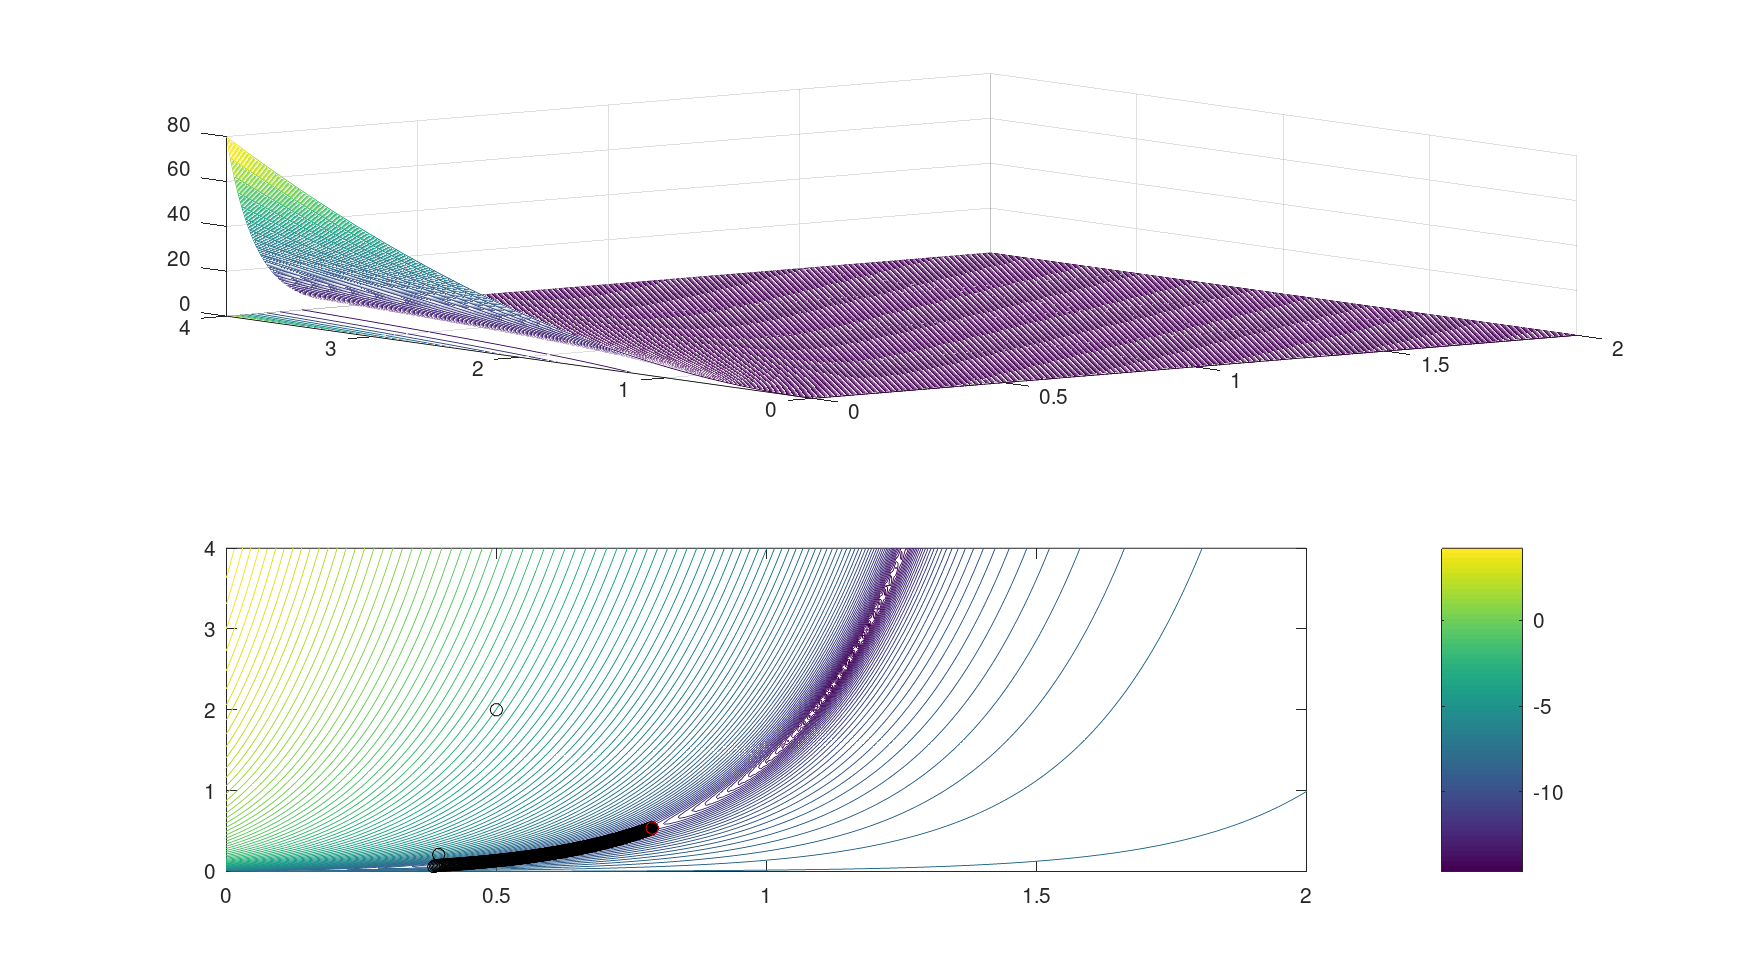
\includegraphics[width=0.7\textwidth]{contourExo2NewtonVariable.png}
                \caption{Convergence pour une direction de Newton avec pas variable}
            \end{figure}
            
             \begin{figure}[H]
                \centering
                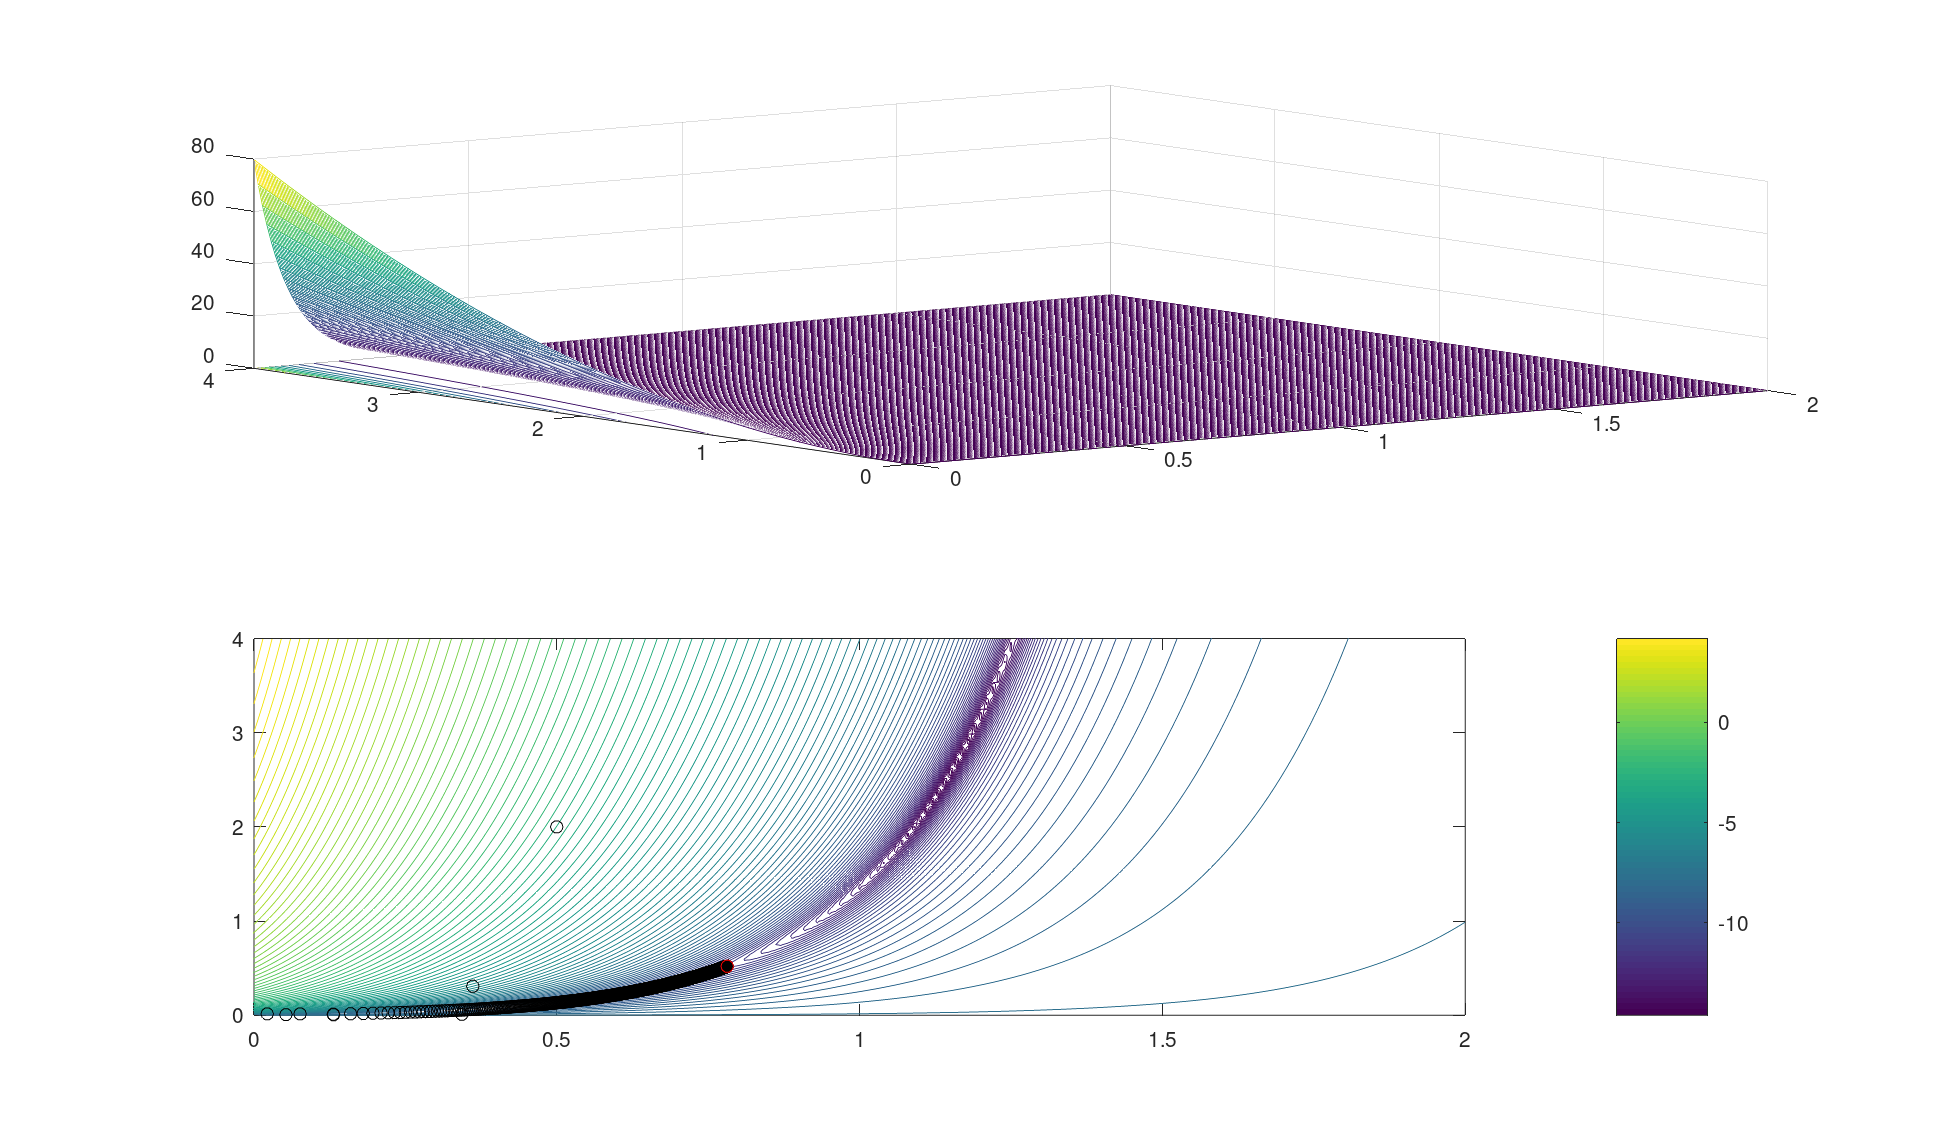
\includegraphics[width=0.7\textwidth]{contourExo2Newton.png}
                \caption{Convergence pour une direction de Newton avec pas fixe}
            \end{figure}
    }
    
    \item{On peut reprendre les valeurs finales dans un tableau en prenant $x_0=[0.5; 2]$:

    	\begin{table}[H]
                \begin{tabularx}{\textwidth}{|l|X|X|X|}
                    \hline
                    Méthode & Nombre d'itérations & Temps (s) & Valeur finale \\
                    \hline
                    Descente de plus forte pente & 1002 & 2 & (1.10, 2.08) \\
                    \hline
                    Gradient conjugué & 1002  &  10.7 & (1.11, 2.15)\\
                    \hline
                    Newton &  1002 & 5.9 & (0.79, 0.54) \\
                    \hline
                    BFGS & 39 & 0.38 & (1.15, 2.55)\\
                    \hline
                \end{tabularx}
            \end{table}
    }
    
    \item{En prenant les différents xh, on obtient la caractéristique théorique  suivante en rouge par rapport à celle de mesure en bleue:
   	 \begin{figure}[H]
                \centering
                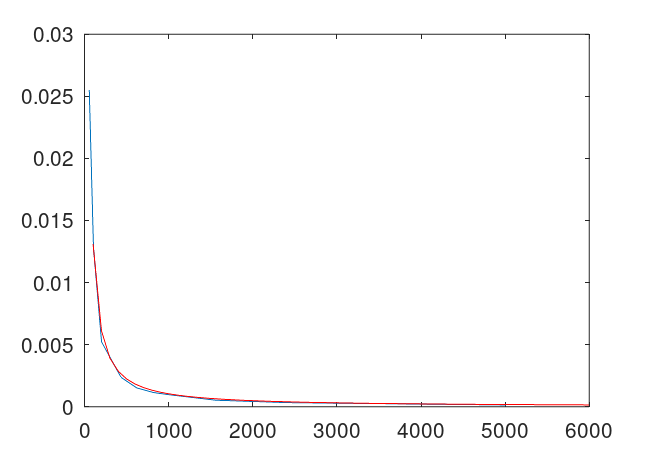
\includegraphics[width=0.7\textwidth]{contourExo2GradientVariableCourbe.png}
                \caption{Caractéristiques théorique en et expérimentale pour $xh = [1.10, 2.08]$ }
            \end{figure}
            
            \begin{figure}[H]
                \centering
                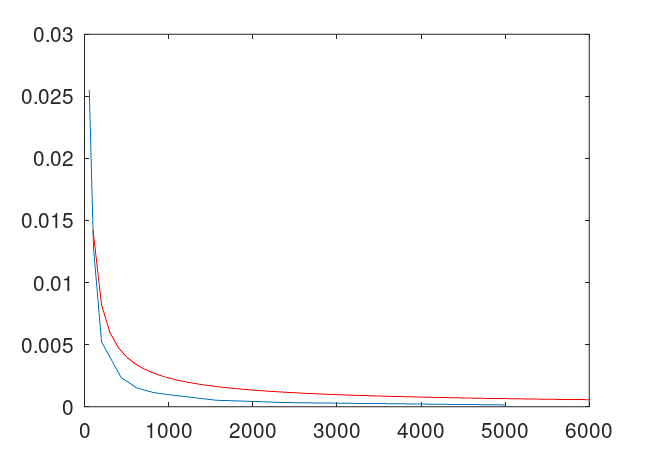
\includegraphics[width=0.7\textwidth]{contourExo2NewtonVariableCourbe.png}
                \caption{Caractéristiques théorique en et expérimentale pour $xh = [0.79, 0.54]$ }
            \end{figure}
        }
\end{enumerate}

\newpage
\section{Débruitage d’un signal par minimisation d ’un critère composite}

\subsection{Simulation des signaux}

\begin{enumerate}

    \item{
            Simulons une réalisation du vecteur $x$ similaire au spectre vibrationnel
            d'une molécule chimique.

            \begin{figure}[H]
                \centering
                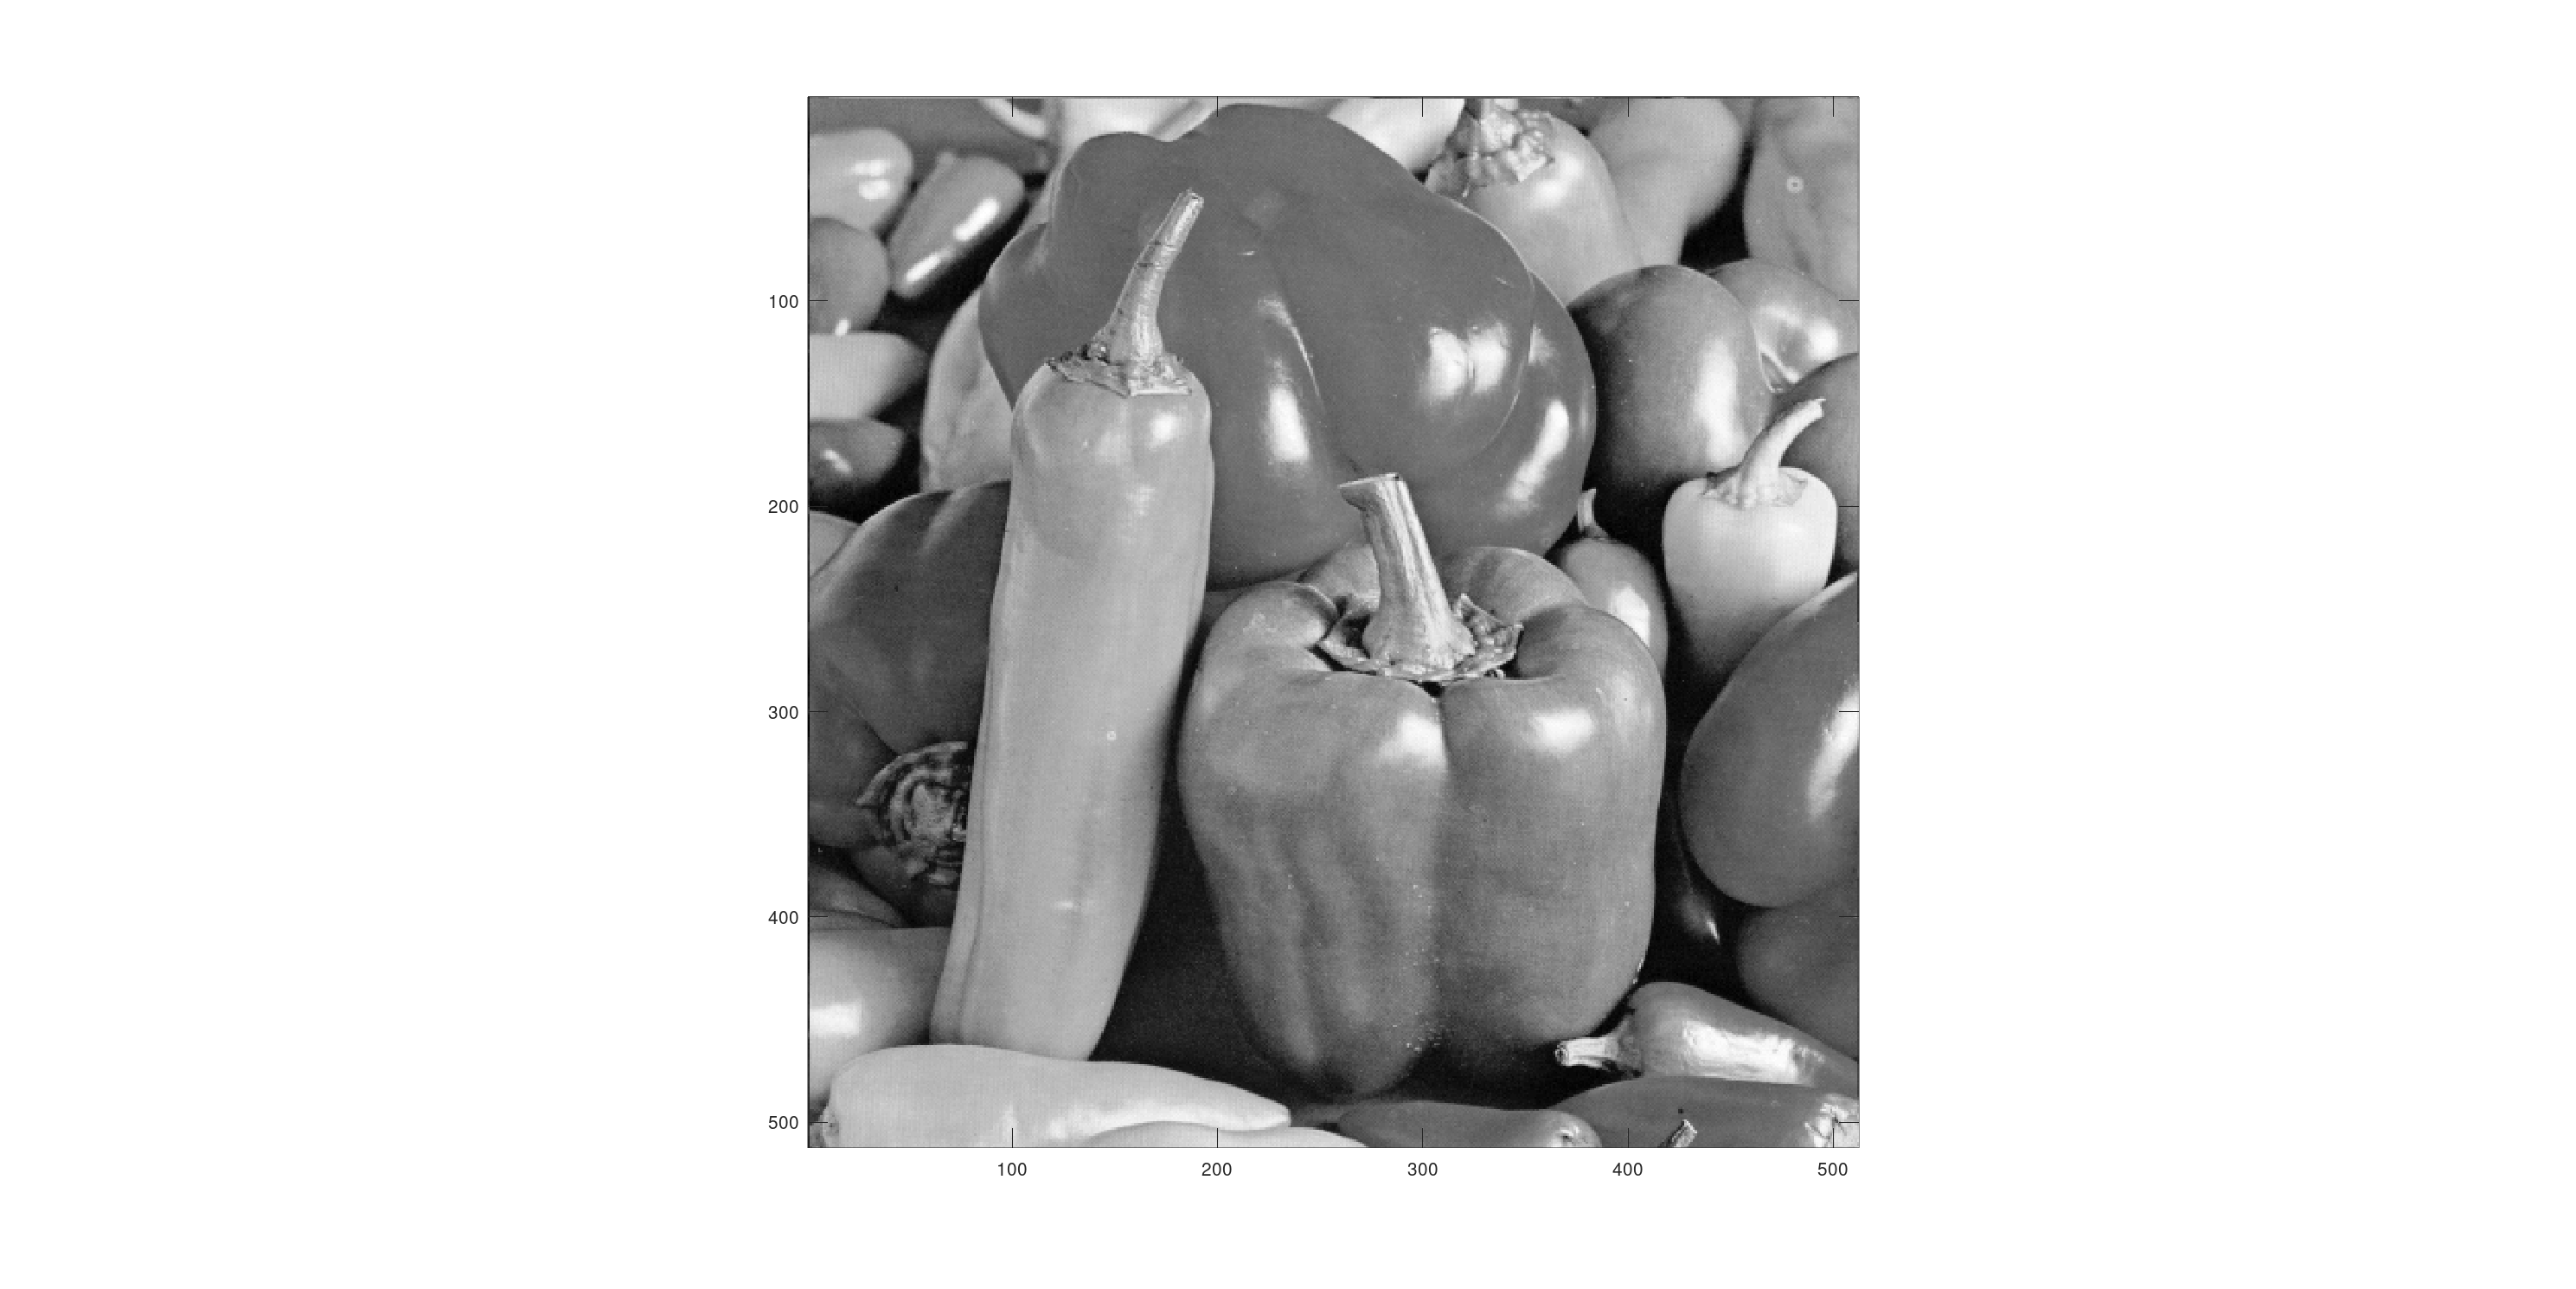
\includegraphics[width=0.7\textwidth]{ex3_1}
                \caption{Signal $x$}
            \end{figure}
        }

    \item{
            Après calcul on obtient une variance égale à $\frac{E_x}{100}$.
        }

    \item{Le signal en présence de bruit à l'allure suivante :

            \begin{figure}[H]
                \centering
                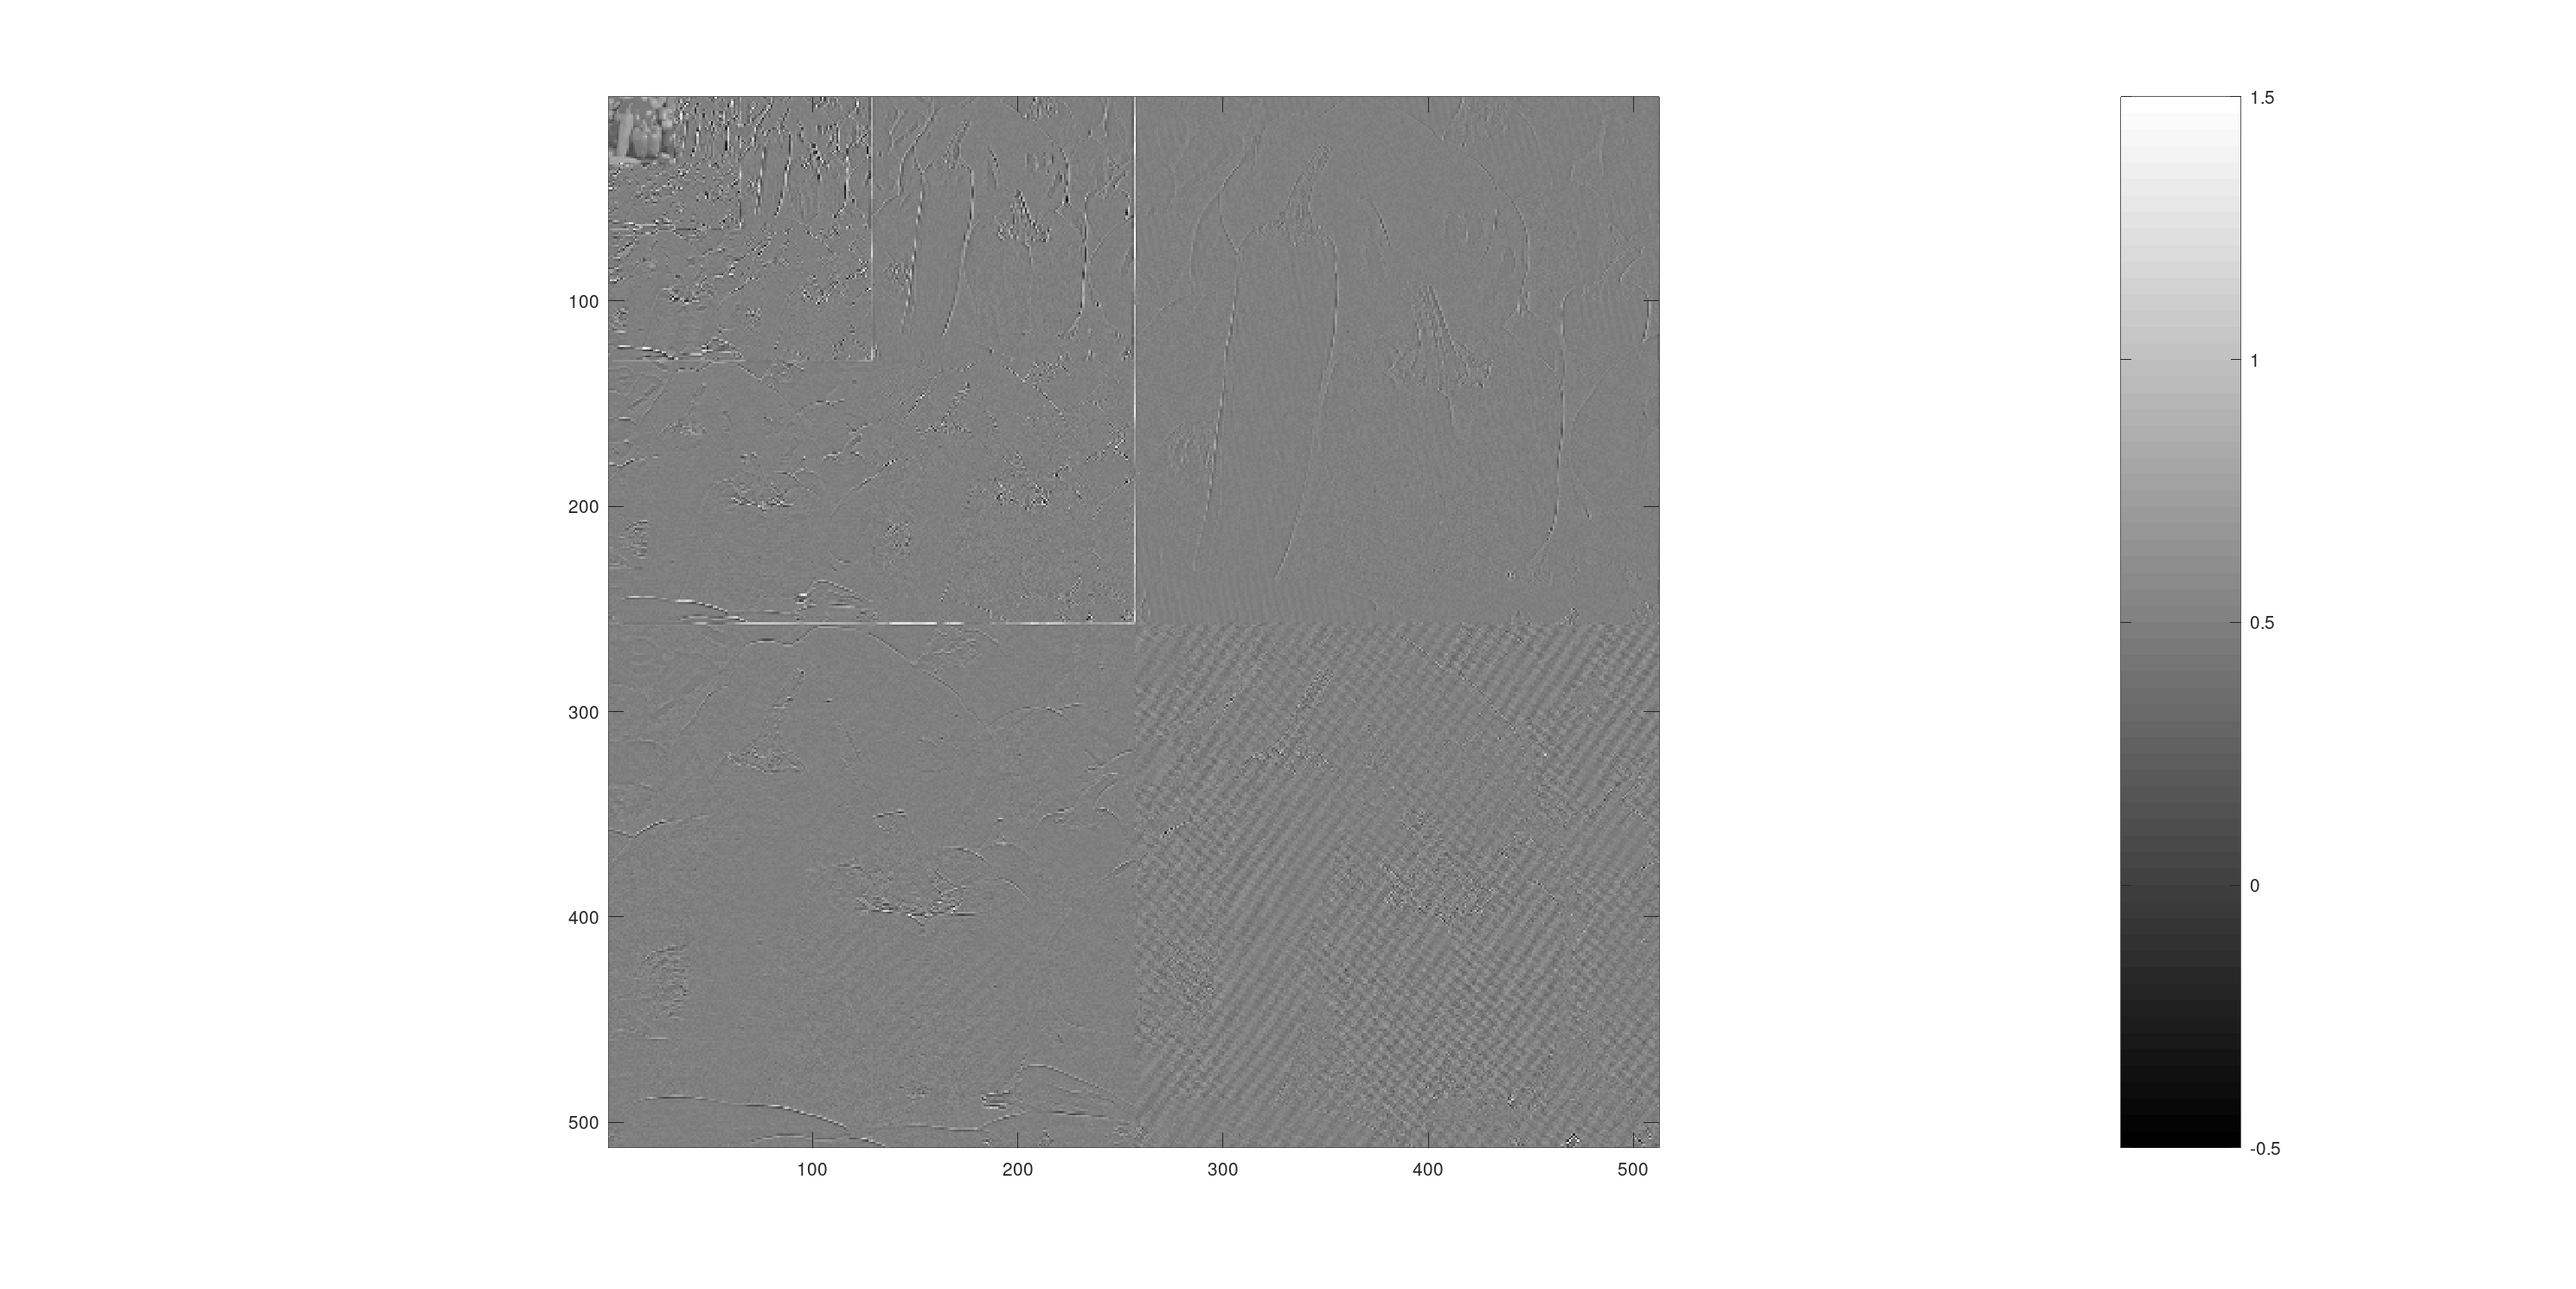
\includegraphics[width=0.7\textwidth]{ex3_2}
                \caption{Signal bruité}
            \end{figure}
        }

    \item{Le modèle de mesure peut s'écrire sous la forme $y = Hx + e$ avec $H = I_n$.}

\end{enumerate}

\subsection{Débruitage du signal}

\begin{enumerate}

    \item{Par minimisation d'un critère de moindre carré on obtiendrait une solution
            égale au signal bruité lui même ce qui n'est pas voulu, il faut introduire
            un autre critère.
        }

    \item{D est une matrice bidiagonale composée de 1 sur la diagnoale principale et
            de -1 sur la diagonale inférieure.

            On a $\nabla f_1(x) = (D + D^T)x$ Or on montre que $D + D^T$ est inversible
            donc la solution est obtenue pour $x^* = (0, \dots, 0)$ ($f_1$ est à valeurs
            positives c'est donc bien un minimum).
        }

    \item{La solution du problème d'optimisation du critère $f_\lambda$ est : 

            $$x^* = (I + \lambda D^T D)^{-1}y$$

            En utilisant une méthode de plus forte pente à pas variable et pour
            $lambda = 0.5$, on obtient les résultats suivants :

            \begin{figure}[H]
                \centering
                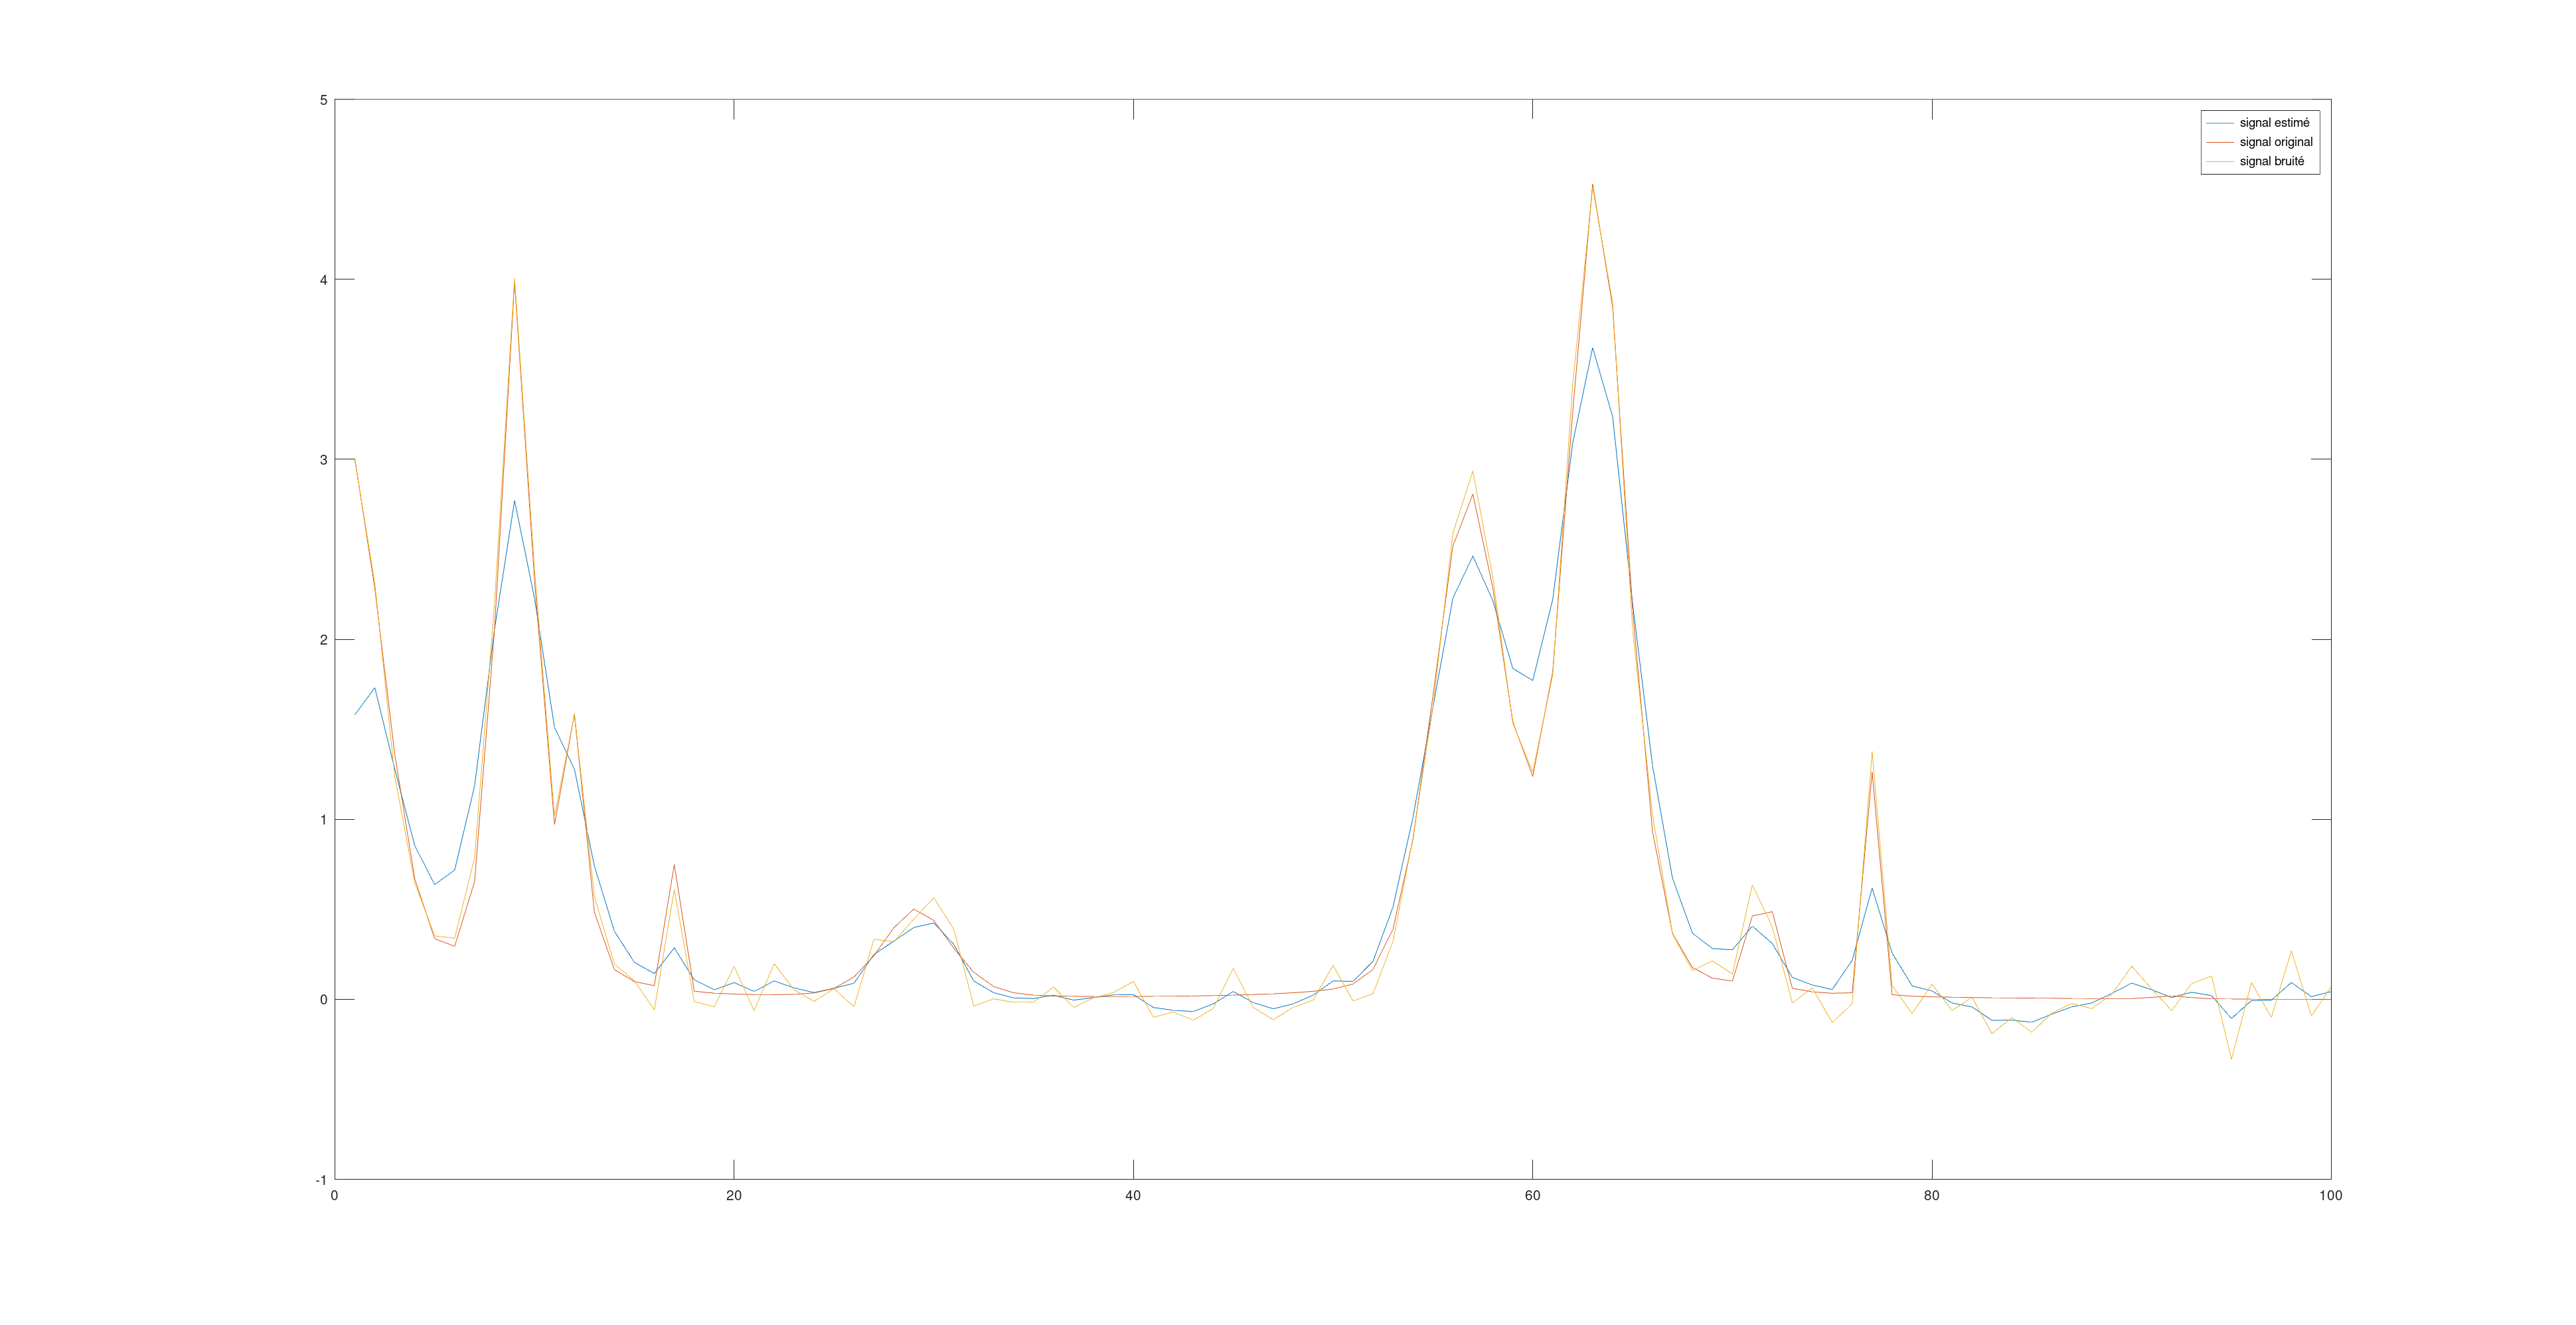
\includegraphics[width=\textwidth]{ex3_3}
                \caption{Résultats pour $\lambda = 0.5$}
            \end{figure}
        }

    \item{
            Représentons l'évolution de l'erreur pour différentes valeurs de \lambda :

            \begin{figure}[H]
                \centering
                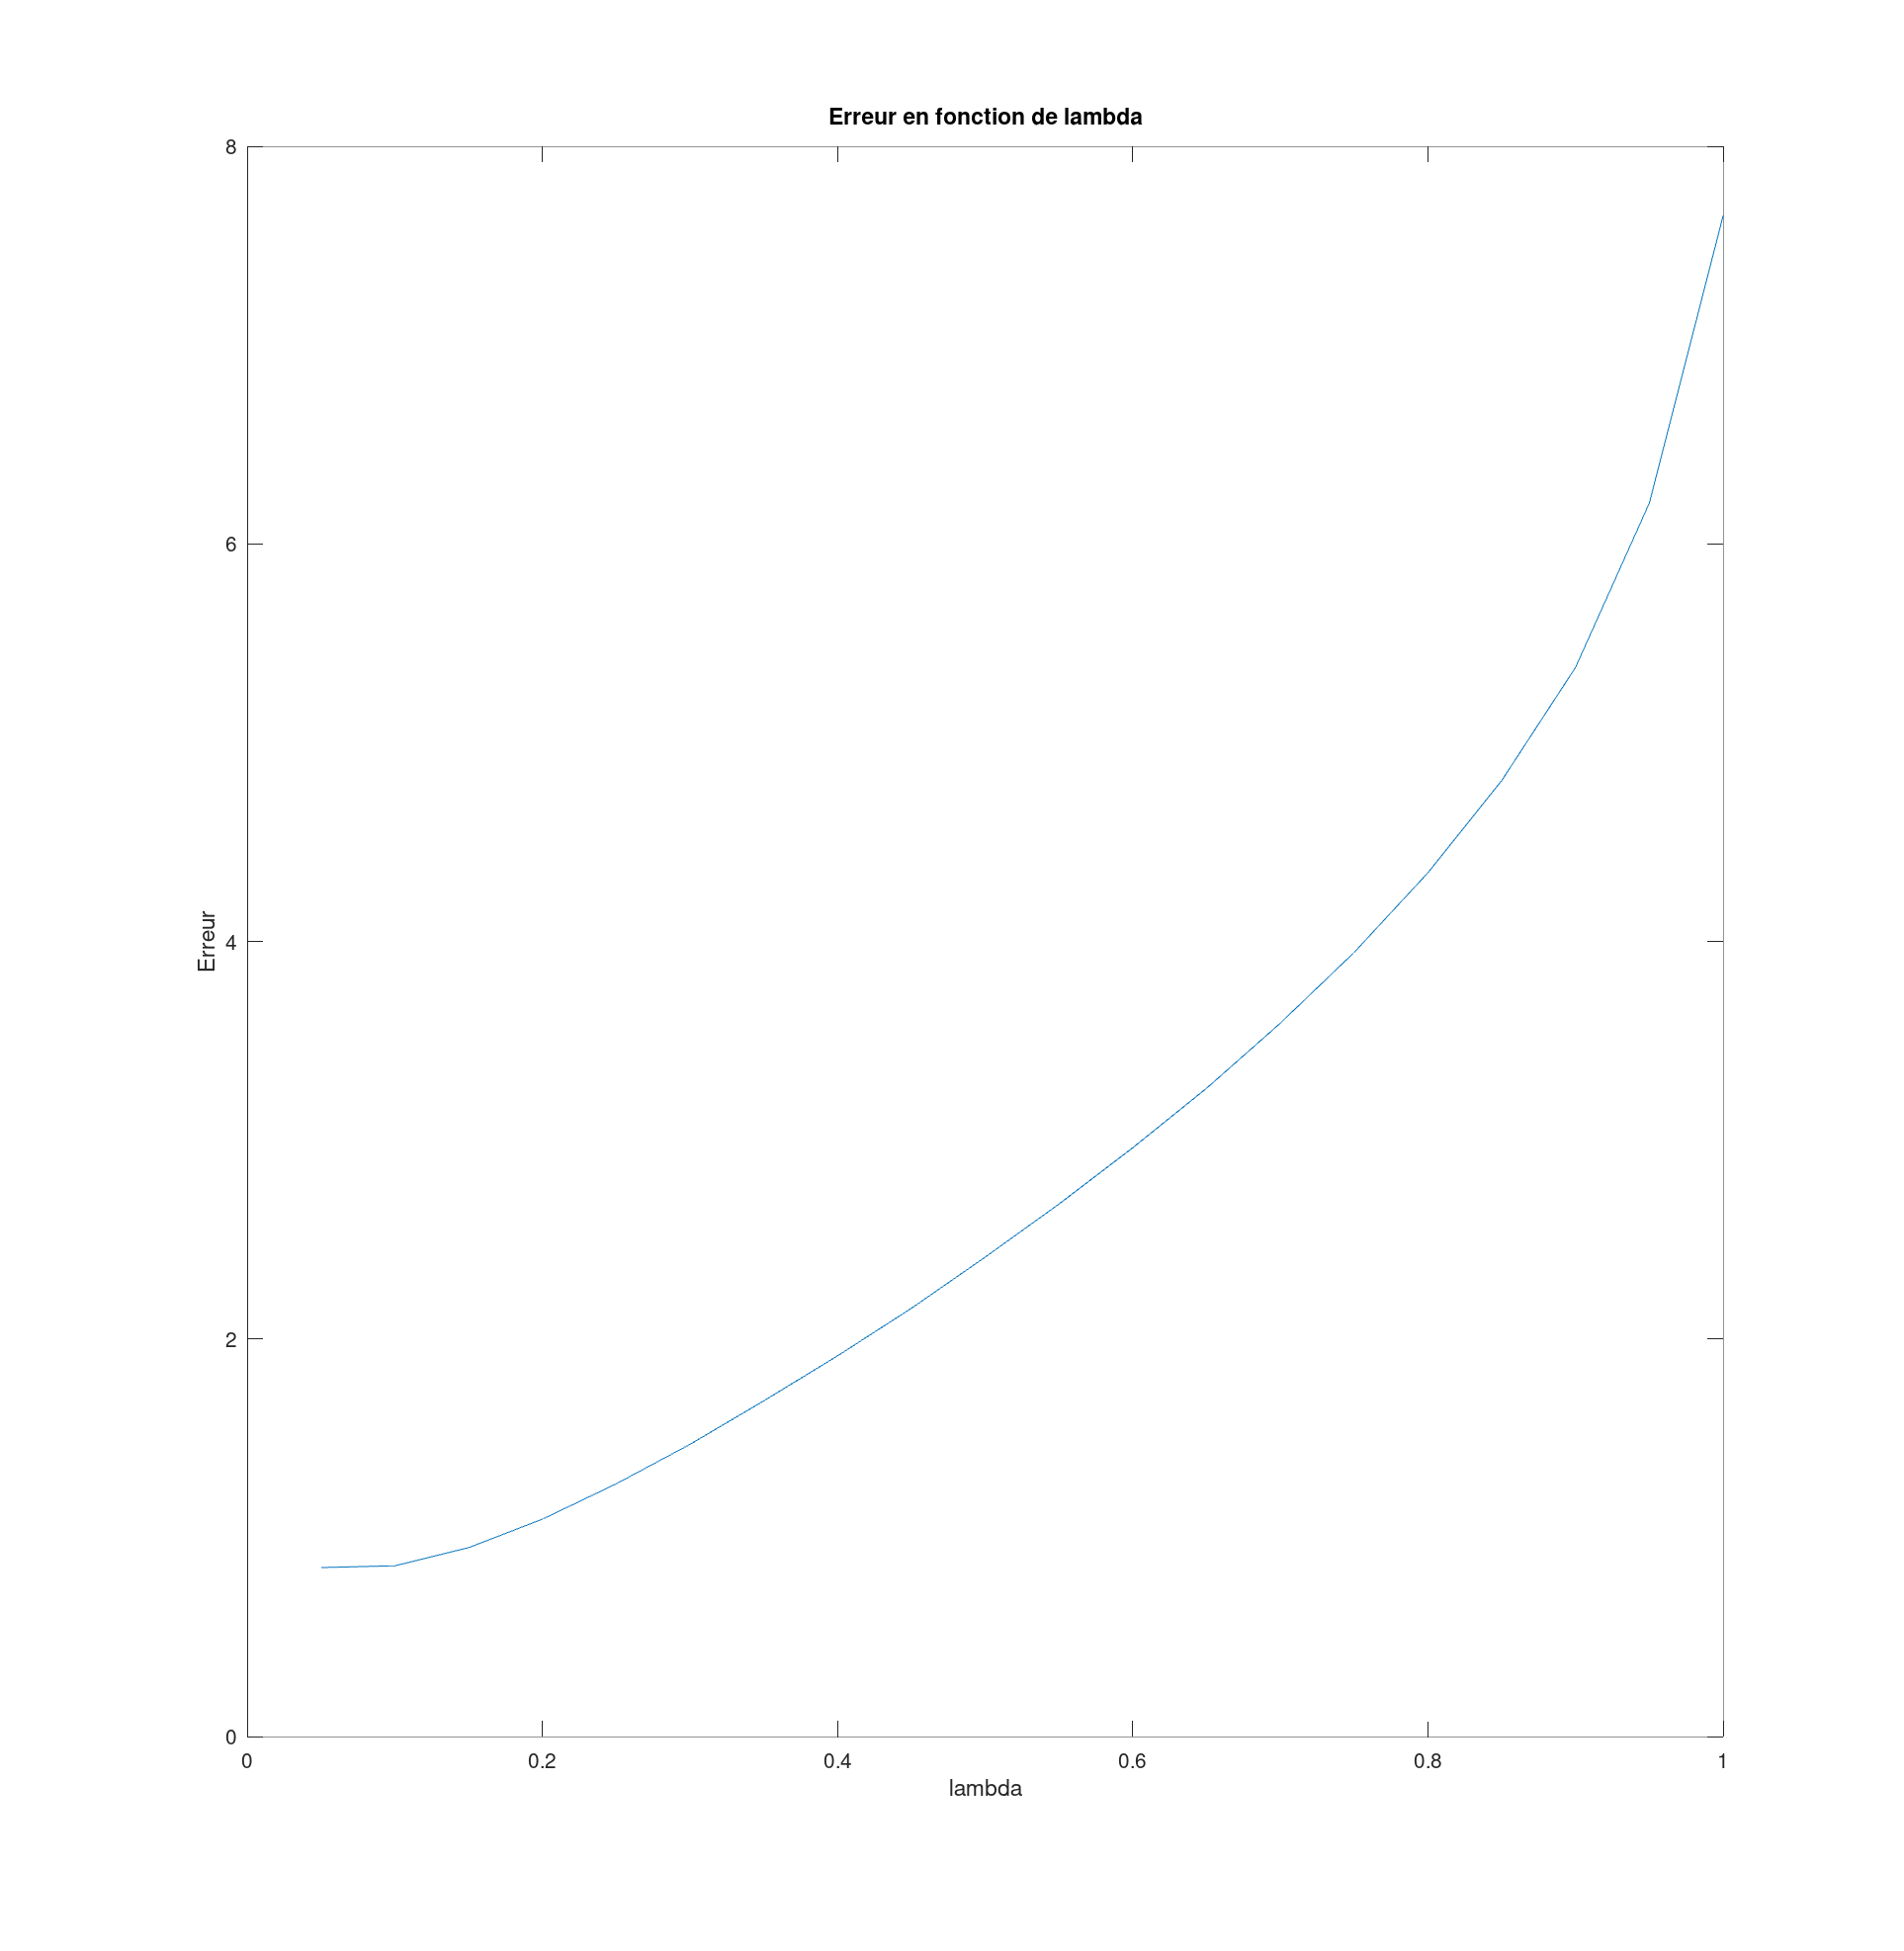
\includegraphics[width=0.7\textwidth]{ex3_4}
                \caption{Évolution de l'erreur en fonction de \lambda}
            \end{figure}

            En terme d'erreur d'estimation, les meilleurs résultats sont obtenus pour
            de faibles valeurs de lambda, c'est-à-dire pour un problème de minimisation
            de $f_0$ plus important que celui de la minimisation de $f_1$, cependant
            comme précisé en 2. nous n'obtiendrons pas un signal debruité pour ces
            valeurs de $\lambda$. Il faut prendre en compte les deux contraintes.
        }

    \item{
            Traçons les valeurs de $f_0$ en fonction de celles de $f_1$ :

            \begin{figure}[H]
                \centering
                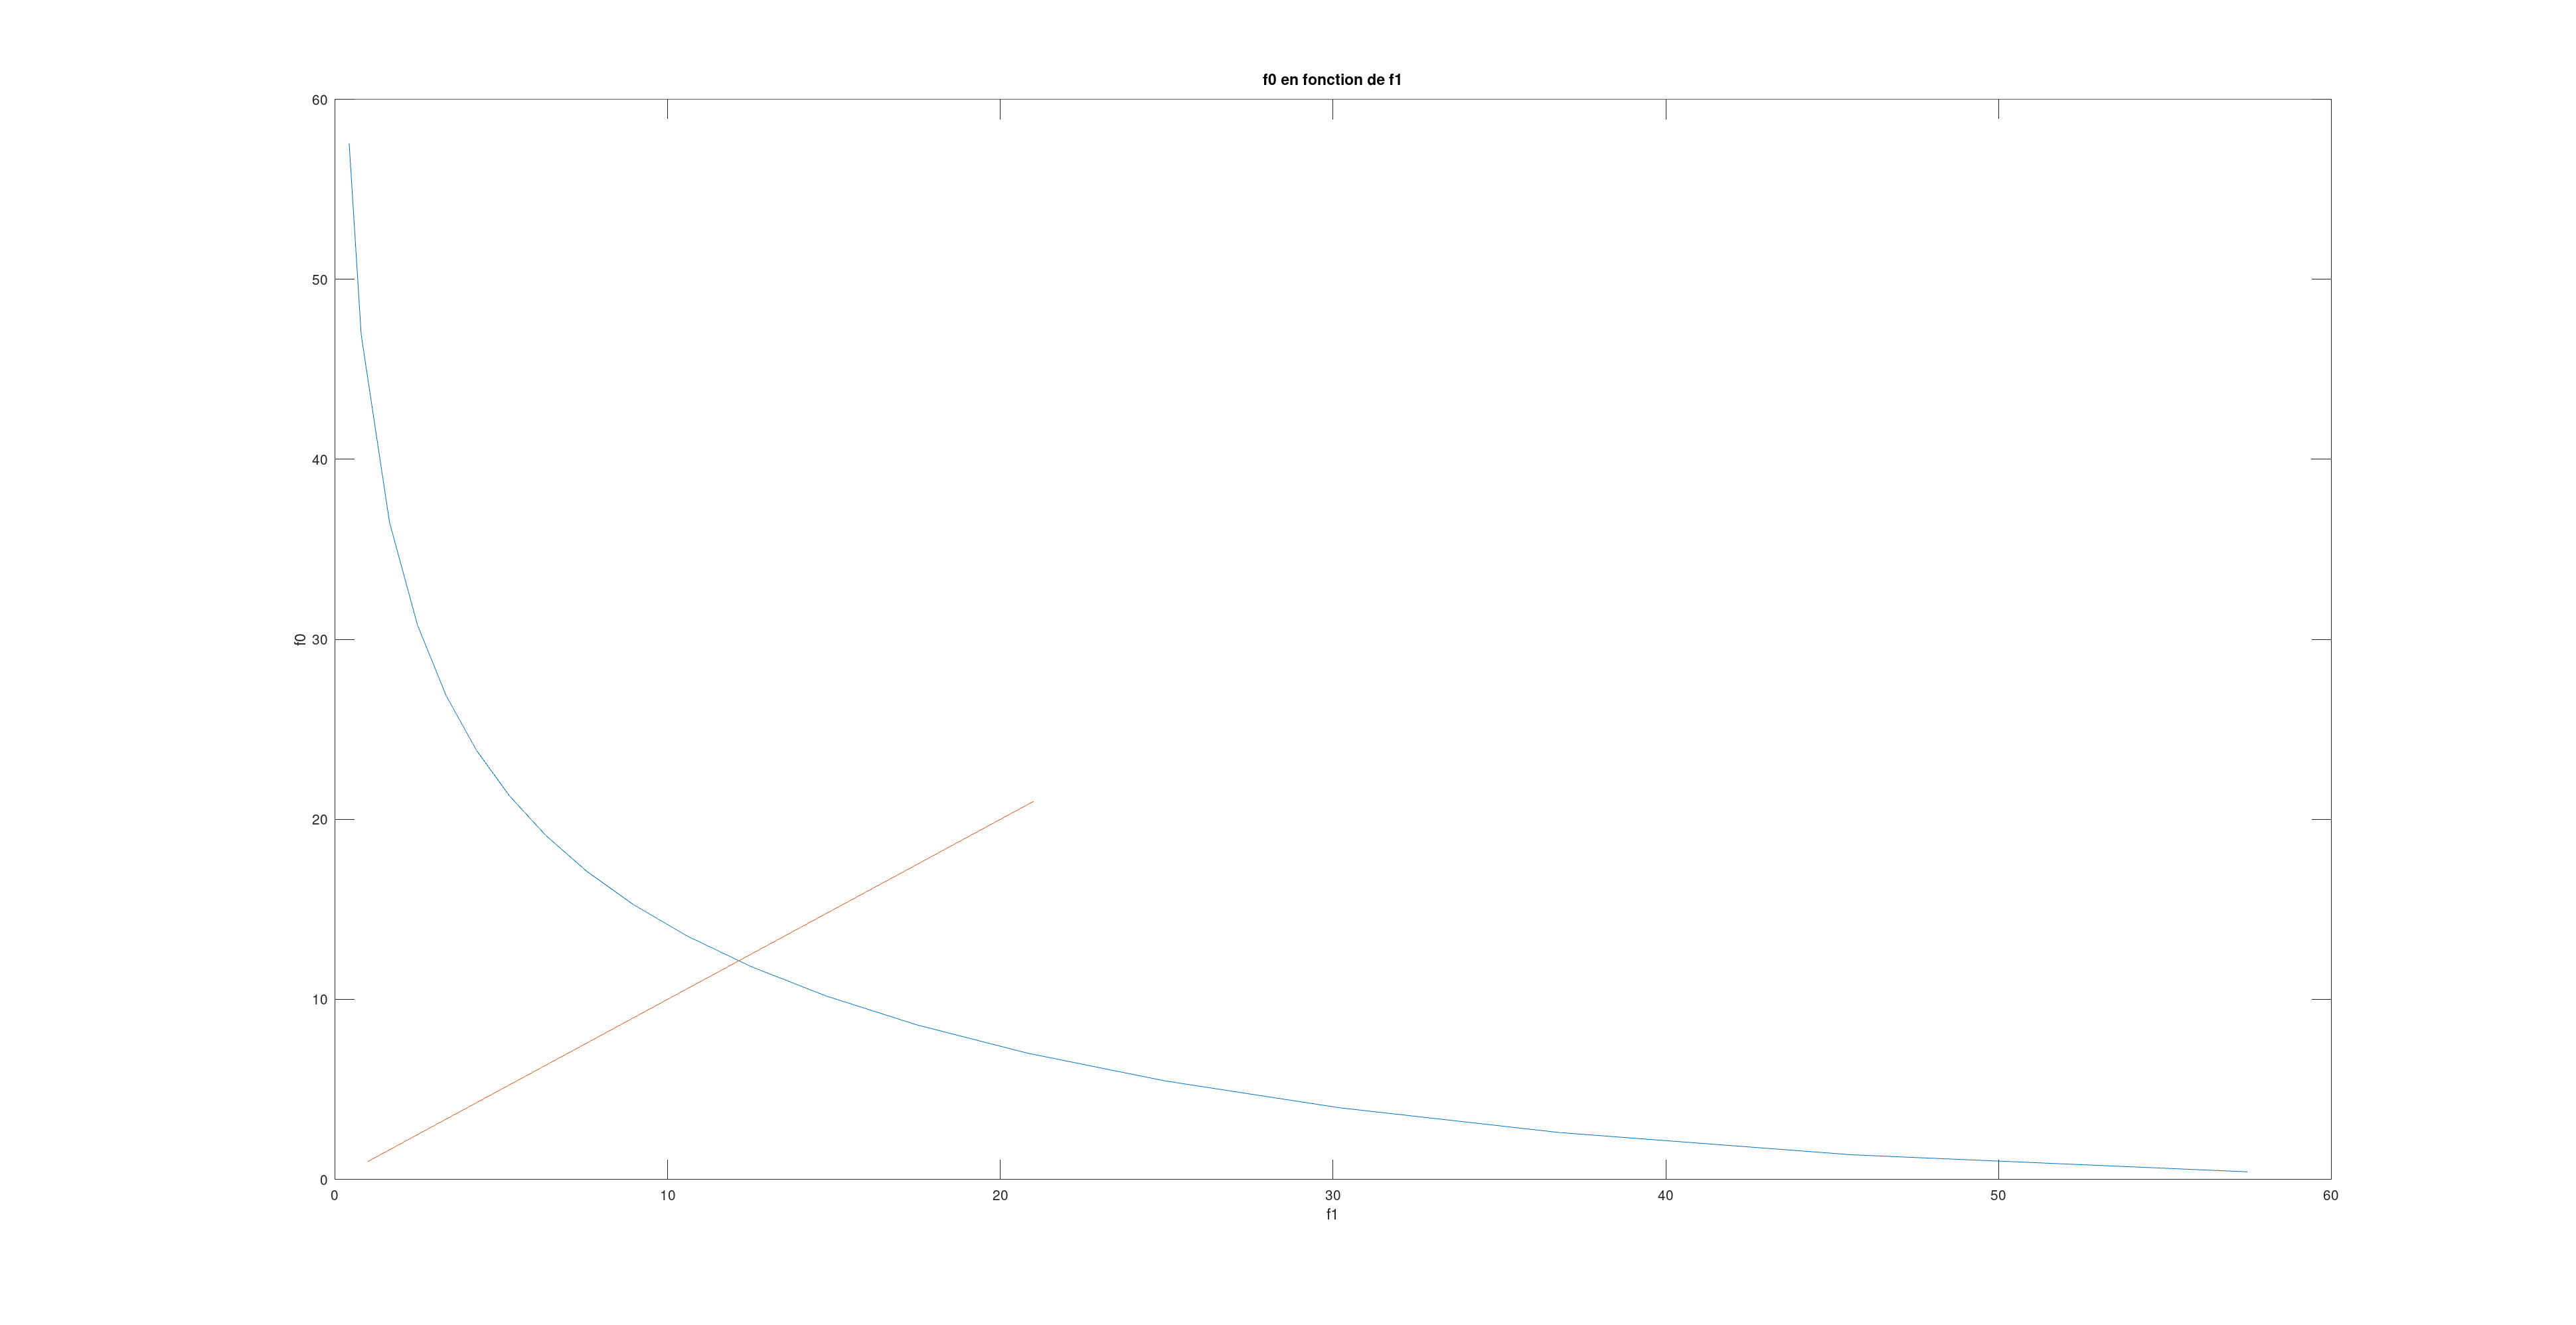
\includegraphics[width=\textwidth]{ex3_5}
                \caption{Valeurs de $f_0$ en fonction de celles de $f_1$}
            \end{figure}

            On peut considérer que la meilleure valeur de $\lambda$ correspond au point 
            d'intersection de la courbe avec la première bissectrice. En effet, 
            on accorde dans ce cas la même importance aux deux critères.

            On obtient alors pour valeur optimale : $\lambda = 0.45$.
        }

\end{enumerate}

\newpage

\begin{appendices}

    \section{Minimisation de la fonction de Rosenbrock}

    \subsection{\texttt{rosenbrock.m}}

    \lstinputlisting[language=Matlab]{../rosenbrock.m}

    \subsection{\texttt{optimdescent.m}}

    \lstinputlisting[language=Matlab]{../optimdescent.m}

    \subsection{\texttt{main\_tpcsopt\_optim1.m}}

    \lstinputlisting[language=Matlab]{../main_tpcsopt_optim1.m}

    \subsection{\texttt{visualisation.m}}

    \lstinputlisting[language=Matlab]{../visualisation.m}

    \subsection{\texttt{comparaison.m}}

    \lstinputlisting[language=Matlab]{../comparaison.m}

    \section{Ajustement d'une courbe non-linéaire}

    \subsection{\texttt{capteur.m}}

    \lstinputlisting[language=Matlab]{../capteur.m}

    \subsection{\texttt{visualisation\_2.m}}

    \lstinputlisting[language=Matlab]{../visualisation_2.m}

    \subsection{\texttt{visualisation\_3.m}}

    \lstinputlisting[language=Matlab]{../visualisation_3.m}

    \section{Débruitage d'un signal par minimisation d'un critère composite}

    \subsection{\texttt{ex3.m}}

    \lstinputlisting[language=Matlab]{../ex3.m}

    \subsection{\texttt{critere\_debruitage.m}}

    \lstinputlisting[language=Matlab]{../critere_debruitage.m}

\end{appendices}

\end{document}
